\documentclass[12pt]{article}
\usepackage{tocloft}% to configure the ToC <<<<<
\setlength{\cftsecnumwidth}{4.5ex}% set the width to the section number in the ToC <<<<<
\renewcommand{\thesection}{\Roman{section}.} 
\renewcommand{\thesubsection}{\quad \Alph{subsection}.}
\renewcommand{\thesubsubsection}{\qquad \roman{subsubsection}.}

\usepackage[style=authoryear,bibencoding=auto,strict,backend=biber,natbib,maxcitenames=2]{biblatex}

\usepackage{amssymb,amsmath,amsfonts,bbm,bm,eurosym,geometry,ulem,graphicx,color,xcolor,setspace,sectsty,comment,float,caption,pdflscape,subfigure,array,hyperref}
\usepackage{xurl}
\usepackage[font=bf]{caption}
\usepackage[bottom]{footmisc}

\hypersetup{
    colorlinks,
    linkcolor={black},
    citecolor={blue!35!black},
    urlcolor={blue!35!black}
}
\addbibresource{bibliography.bib}

\normalem

\onehalfspacing

\geometry{left=1.0in,right=1.0in,top=1.0in,bottom=1.0in}

\begin{document}
\begin{titlepage}
\title{Staggered Difference-in-Differences Estimation for Antitrust Analysis: A Review of Literature and Recommendations for Practitioners}
\author{Hassan Faghani\thanks{Berkeley Research Group (BRG).} \and Steven VanOmmeren\thanks{
BRG. \\\\ We thank colleagues at BRG for providing helpful comments in forming this paper, including Daniel Boada, Robin Cantor, Joshua Hochberg, and Matthew Vaughn, as well as the insightful input of anonymous referees. The views expressed herein are solely those of the authors, who are responsible for the content, and do not necessarily represent the views of BRG. Any and all mistakes are our own. A replication package for our analysis is available at \url{https://github.com/svanomm/faghani-vanommeren-2024/}.
}
}

\date{\today}
\maketitle
\begin{abstract}
\noindent 
The aim of this paper is twofold: first, we discuss literature developments surrounding difference-in-differences (DiD) methods with staggered treatment mechanisms. Second, we provide a resource for sound DiD analysis in antitrust expert testimony in light of these developments. We review relevant papers and their most important conclusions. We then discuss the antitrust implications of three important topics: parallel trends, the not-yet-treated group, and data with customer entry and exit. We supplement this discussion with Monte Carlo analysis, in which we compare the performance of DiD estimators and quantify certain types of bias. Finally, we discuss the sensitivities and robustness checks that should underlay expert testimony going forward. DiD theory has come a long way in the academic literature since the 2010s, and we distill that knowledge into what we consider to be the standards for robust DiD results going forward.\\
\vspace{0in}\\
\noindent\textbf{Keywords:} difference-in-differences, staggered treatment, heterogeneity, antitrust
\vspace{0in}\\
\noindent\textbf{JEL Codes:} C18, C52, L40\\

\bigskip
\end{abstract}
\setcounter{page}{0}
\thispagestyle{empty}
\end{titlepage}
\pagebreak \newpage


\tableofcontents

\doublespacing

\newpage
\section{Introduction} \label{sec:introduction}
Understanding the effects of policy changes is among the fundamental problems of applied social sciences. In economic and legal studies, one of the most popular techniques for measuring the effects of policy changes is difference-in-differences (DiD) analysis.\footnote{We wrote a high-level summary of DiD and the literature developments in early 2023. This paper provides more econometric detail and cites several papers that have been published since our previous article. \url{https://www.law360.com/articles/1568455/the-difference-in-differences-antitrust-analysis-is-evolving}.}  At its core, DiD is relatively simple to understand, contributing to its popularity. In DiD, a group of entities, such as firms, stores, or customers, that have been affected by an event of interest are compared against a similar group of entities that were not affected. We then analyze the trend over time of this difference---a difference (over time) in differences (between the affected and unaffected). DiD essentially combines two common impact analysis methods (yardstick and before-after analysis) to yield a more robust estimate.\footnote{The ``yardstick'' method compares a group of affected units to unaffected units, but does not incorporate a trend over time. ``Before-after analysis'' does not compare affected units to unaffected units.} The underlying assumption is that the studied policy is the only relevant change between the two groups once the treatment starts. The affected group is referred to as the “treatment group,” the unaffected is the “control group,” and the impact we aim to recover is called the ``treatment effect.''\footnote{In this paper, we use ``treatment effect'' interchangeably with the average treatment effect on the treated (ATT). This is the average effect that the policy causes on the treatment group units only, as opposed to the hypothetical effect that the treatment would have on both the treatment \textit{and} control groups.} A simple DiD visualization is shown in Figure \ref{fig:did-diagram}.
\begin{figure}[H]
    \centering
    \caption{Example of Simple DiD Analysis}
    \includegraphics[width=5in]{Figures/Diff in Diff Diagram.PNG}
    \label{fig:did-diagram}
    \vspace{5mm}
    \footnotesize \begin{singlespace*}
        \parbox{5.5in}{A hypothetical DiD example. Here, the treatment group experiences a policy change starting at the dashed vertical line. To calculate the average treatment effect, we compare the difference pre-/post-policy for the control group with that of the treatment group. The dashed blue line represents how the treatment group would have moved if it followed the control group’s behavior in the post-policy period.}
    \end{singlespace*}
\end{figure}
\noindent
DiD is commonly used in antitrust litigation analysis for estimating the economic impact of alleged anticompetitive behavior. For example, it was used to estimate class-wide overcharges and damages in the market for data management systems.\footnote{\textit{In re Dealer Management Systems Antitrust Litigation}, 581 F.Supp.3d 1029 (N.D.Ill., 2022). Part of the challenge against one of the Plaintiff experts' reliability involved assessing a violation of the parallel trends assumption. \textit{Id} at 69.}  DiD was used to estimate overcharges to manufacturers from an alleged conspiracy to raise prices of coupon-processing fees.\footnote{\textit{Mr. Dee's Inc. v. Inmar, Inc.}, 2021 WL 4224720 (M.D.N.C., 2021), at *5. Plaintiff’s expert supplemented the DiD analysis with both a before-after (difference over time) and yardstick approach (contemporaneous difference between treatment and control). }  DiD measured whether Staples stores’ prices were lower when they faced local competition from Office Depot.\footnote{\citet{ashenfelter2004}, Equations 2 through 5 (discussing  \textit{Federal Trade Commission v. Staples, Inc.}, 970 F. Supp. 1066 (D.D.C., 1997)). While not described as such, these regressions are forms of two-way fixed effects (TWFE) models, which are a type of DiD analysis.}  And it was used to assess “whether and to what extent NorthShore's post-merger price increases were the result of increased market power resulting from the merger [with Highland Park Hospital].”\footnote{\textit{In re NorthShore Univ. HealthSystem Antitrust Litig.}, No. 07-cv-4446, 2018 WL 2383098, at *2, citing \textit{Messner}, 669 F.3d, at 818. Interestingly, the experts debated whether Plaintiff’s DiD analysis was valid in the presence of non-uniform (i.e. heterogeneous) price increases, a subject of the literature we discuss.} Additionally, the antitrust academic literature has used DiD extensively to measure the economic impact of mergers, market entry, and other competition-related behavior. A summary of antitrust applications of DiD is shown below.  

\begin{table}[htbp]\centering
\def\sym#1{\ifmmode^{#1}\else\(^{#1}\)\fi}
\caption{Examples of Antitrust Difference-in-Differences Analysis}
\label{tab:antitrust-did}
\def\sym#1{\ifmmode^{#1}\else\(^{#1}\)\fi}
\scalebox{0.7}{
\begin{tabular}{lcccc}
\hline\hline

                    Paper/Case & TWFE? & Staggered? & Time-Varying & Robust Estimators  \\
                    & & & Covariates? & Used? \\
                    \hline 
                    \citet{brot2024toolittle}                          & Yes & Yes & Yes & Yes \\
                    \citet{hosken2022vertical}                         & Yes & Yes & No  & No \\
                    \citet{prager2021employer}                         & Yes & Yes & Yes & Yes \\
                    \textit{Mr. Dee's Inc. v. Inmar, Inc.} (2020)      & No  & No  & Yes & No \\
                    \textit{In re Dealer Management Systems} (2019)    & Yes & No  & Yes & No \\
                    \citet{carlton2019legacy}                          & Yes & Yes & Yes & No \\
                    \textit{Shane Group, Inc. v. BCBS Michigan} (2013) & No  & \;Yes$^1$ & Yes & No   \\
                    \textit{Messner v. Northshore} (2012)              & Yes & No  & Yes & No \\
                    \citet{ashenfelter2010effect}                      & \;Yes$^2$ & No  & No  & No \\
                    \citet{goolsbee2008incumbents}                     & Yes & Yes & Yes & No \\
                    \citet{taylor2005michigan}                         & No  & No  & \;Yes$^3$ & No \\
                    \citet{berry2001mergers}$^4$                       & No  & No  & Yes & No \\
                    \textit{FTC v. Staples, Inc.} (1997)               & Yes & Yes & Yes & No \\
\hline\hline
\multicolumn{5}{l}{\footnotesize Note: for court cases, the year shown here is when the relevant DiD expert report was written.} \\
\multicolumn{5}{l}{\footnotesize 1. While the treatment effect was staggered, the expert ran separate regressions for each treated unit.} \\
\multicolumn{5}{l}{\footnotesize 2. The authors used fixed effects for each month of the year, rather than a traditional TWFE's fixed effects} \\ 
\multicolumn{5}{l}{\footnotesize \phantom{2. }for each time period in the data.}\\
\multicolumn{5}{l}{\footnotesize 3. The authors used three indicator variables to control for unrelated events that could affect the outcome variable.}\\
\multicolumn{5}{l}{\footnotesize 4. DiD was used as a sensitivity, not a main model in this paper.}\\
\end{tabular}
}
\end{table}


DiD isolates the average effect of a policy change only under certain assumptions. The most prominent and contentious assumption in antitrust analysis is that the treatment group would have followed the same relative path as the control group absent the policy change.\footnote{Relatedly, DiD models also assume that, unless explicitly accounted for, treatment units are not affected by the treatment effects of other units around them. In other words, there can be no spillover effects from treatment. As we discuss in \hyperref[sec:notyettreated]{Section V.B}, staggered treatment can make this assumption more questionable.} This assumption is called the \textbf{parallel} or \textbf{common trends assumption}. Equivalently, DiD attributes any change in the treatment group as being due to the policy change; it assumes that all other meaningful events are controlled for. Failing the parallel trends assumption can call into question the validity of DiD results and makes causal interpretation difficult.\footnote{\label{footnote:daubert} The parallel trends assumption is often a central topic of critique in \textit{Daubert} challenges of DiD antitrust analysis. The \textit{Daubert v. Merrell Dow Pharmaceuticals, Inc.}, 509 U.S. 579 Supreme Court decision in 1993 established new guidelines on the admissibility of expert testimony. \citet{langenfeld2010daubert}, pp. 2-3 (``In addition to requiring the witness be qualified to offer testimony, this revision resulted in courts applying three general rules to determine the admissibility of expert testimony including: (1) the testimony is based upon sufficient facts or data, (2) the testimony is the product of reliable principles and methods, and (3) the witness has applied the principles and methods reliably to the facts of the case."). Successful \textit{Daubert} challenges can result in expert testimony being partially or entirely excluded from evidence.} In practice, it can be difficult to perfectly satisfy the parallel trends assumption. With non-experimental data, control groups may have some observable differences with the treatment group. However, econometricians have still extracted useful information from DiD models, adding caveats about uncertainty to their results rather than rejecting them entirely. We discuss how parallel trends tests and assumptions are affected by developments in the DiD literature in more detail in \hyperref[sec:parallel-trends]{Section V.A}.

Research questions are often more complicated than just measuring one average effect, and the nature of the data and policy of interest may further complicate things. To account for these complications, DiD analysis of antitrust conduct is typically implemented with a linear regression, which can control for observable factors and estimate the statistical significance of results. In our experience, DiD models used in expert testimony often include covariates, with the idea that the additional variables ensure that the DiD estimates isolate the impact of the event of interest.

One common complication in a DiD framework is differential treatment timing, where different units affected by the policy or conduct start or end their treatment at different times. A special case of differential treatment timing, where the treatment units remain permanently affected after their treatment, is called \textbf{staggered treatment}.\footnote{We examine binary staggered treatment in this paper, which additionally assumes that the treatment effect is immediate and can only be turned on or off. A non-binary treatment example would be drug trials which give different amounts of the drug to different treatment units. Binary treatment is most common in antitrust work, where we usually have no way of knowing or characterizing “how much” of the treatment is happening. However, certain types of non-binary treatment can be effectively estimated by the methods we discuss here. For example, the ramp-up effects of a conspiracy could be captured by measuring treatment effects over time.}  Staggered treatment designs are common in policy evaluation and antitrust analysis.\footnote{For example, \citet{brot2024toolittle} estimate the average price effect of several hundred hospital mergers between 2010 and 2015.} A representation of a staggered treatment design is shown below in Figure \ref{fig:visual}. Note how in certain years, there are units that have not yet been affected by the policy change (the “not-yet-treated” group), and others who have. DiD analysis in this setting will use the not-yet-treated group, along with the prototypical control group (now called the “never-treated” group), in forming the estimated policy effect. How exactly this works is a focal point of the literature we discuss below.
\begin{figure}[H]
    \centering
    \caption{Representation of Staggered Treatment Mechanism}
    \includegraphics[width=5in]{Figures/Visual Staggered Treatment.PNG}
    \label{fig:visual}
    \vspace{2mm}
    \footnotesize \begin{singlespace*}
        \parbox{5.5in}{In this diagram, each row represents an individual in the data. The first two rows never experience the policy change. The remaining four rows each experience the effects of the policy starting at different times, from 2017 to 2020. In this case, the policy and its treatment effect are staggered across the units.}
    \end{singlespace*}
\end{figure}
Antitrust analysis often includes entities in the treatment and control groups that “enter” or “exit” during the timeframe of the data. For example, analyzing the price effects of hospital mergers would see some hospitals enter the market while others close. This results in ``unbalanced panel'' data, which comes with additional complications in a DiD setting. Unbalanced panels can result in some treatment group units having no ``before'' period to establish an untreated baseline; we call these units the ``always-treated group.'' A representation of a staggered treatment mechanism with an unbalanced panel is shown below in Figure \ref{fig:visual-unbalanced}. We discuss the complications of using such data in \hyperref[sec:unbalanced]{Section V.C below}.
\begin{figure}[H]
    \centering
    \caption{Representation of Staggered Treatment Mechanism with an Unbalanced Panel}
    \includegraphics[width=5in]{Figures/Visual Staggered Unbalanced Treatment.PNG}
    \vspace{2mm}
    \footnotesize \begin{singlespace*}
        \parbox{5.5in}{Example of a staggered treatment mechanism with unbalanced data. Unit 4 has no “before” period and so is part of the always-treated group.}
    \end{singlespace*}
    \label{fig:visual-unbalanced}
\end{figure}
One can imagine many other complications of applied DiD analysis. The important question is: how do these complications interact with our ability to accurately measure the treatment effect? Suppose that a national hospital system acquires several competitors across the country over multiple years. It is likely that price effects following the mergers may change over time as customers and competitors respond to supracompetitive prices. Payors in some areas may negotiate more favorable contracts than others, depending on local competitive conditions. It is also possible that payors who signed a contract prior to the merger are shielded from any price increases until their contract expires. All of these examples require special consideration when performing DiD analysis.

Since the late 2010s, a large body of literature on DiD analysis has appeared which aims to better understand how such complications affect our regression results. Academics have largely confirmed the suspicions of careful applied econometricians by proving that results are biased if we do not account for the studied policy and its effects appropriately.\footnote{For the purposes of this paper, we use the term ``bias'' to refer to the degree to which an estimated effect is different from the true effect it is designed to estimate. Unbiased estimators recover the true effect in expectation.} But of particular interest, research has revealed a bias in DiD estimates inherent to the staggered nature of the treatment mechanism which is often overlooked by practitioners. The literature has provided several alternative estimators that are robust to this and other types of misspecifications, detailed sets of assumptions that underlie their results, and many sensitivities and tests to diagnose issues common to DiD analysis.\footnote{This DiD literature has caught on quickly in the academic space, with some seminal papers already having several thousand citations. It is already a lecture topic in current PhD-level econometrics courses and has been the subject of several conferences, seminars, and special journal issues. The literature is also beginning to enter antitrust expert analysis. The authors have personally encountered the \citet{CS2021} and \citet{goodman-bacon2021a} papers in antitrust expert testimony.}

We review the main developments in DiD literature in \hyperref[sec:literature]{Section II}. \hyperref[sec:analysis]{Section III} summarizes the estimators we think are best suited for antitrust work. Results using a Monte Carlo analysis are reported in \hyperref[sec:analysis]{Section IV}. \hyperref[sec:antitrust]{Section V} further discusses three topics of interest for antitrust practitioners. In \hyperref[sec:conclusion]{Section VI} we conclude.

\section{Forbidden Comparisons and Weighting Issues in Staggered DiD} \label{sec:literature}
It is typical for DiD analyses (in antitrust or otherwise) to use a linear regression with fixed effects to control for confounding factors that might explain changes in an outcome variable such as price.\footnote{``Fixed effects'' are indicator variables for each level of a categorical outcome. For example, a regression with hospital fixed effects would have a separate indicator variable for each hospital in the data, leaving one hospital indicator excluded to avoid collinearity.} In particular, many models include fixed effects for both the time and unit dimensions in the data. These regressions are called ``two-way'' fixed effects or TWFE models and take the following form:
\begin{equation}
    y_{it} = \alpha_i + \lambda_t + \boldsymbol{\gamma}  D_{it} + \beta X_{it} + \epsilon_{it},
\end{equation}
where $y_{it}$ is the outcome of interest, such as price, $\alpha_i$ are unit fixed effects, $\lambda_t$ are time period fixed effects, $D_{it}$ is an indicator variable which is 1 for being actively affected by the policy and 0 otherwise, $X_{it}$ represents other observable variables, and  $\epsilon_{it}$ captures variations in the data that cannot be explained by the model.\footnote{This model specification is referenced in many popular econometric textbooks, including  \citet{angrist2009mostly}, Section 5.2.1; \citet{hansen2022econometrics}, p. 671; and \citet{cameron2020}, pp. 768-770. \\\\ TWFE is considered a “default” DiD specification when there are multiple groups and time periods. This is often a matter of convenience. Rather than identifying which confounding events or characteristics need to be controlled for in the model, TWFE controls for all time-invariant and unit-invariant heterogeneity. But these fixed effects do not control for time-varying events that affect a subset of the units or which vary by unit.} Unlike a classical DiD regression, TWFE regressions will run and estimate a treatment effect when treatment is staggered (i.e. with multiple treatment times).

TWFE models are very common, as detailed by \citet{de2020two}, who found that nearly one in five empirical articles from 2010 to 2012 published in the American Economic Review used the specification to estimate treatment effects.\footnote{\citet{de2020two}, p. 2964.} TWFE models are also often used in antitrust analysis, appearing in both acacdemic studies and in expert testimony.\footnote{As mentioned above, experts in \textit{Federal Trade Commission v. Staples, Inc.} used TWFE models, and we have encountered the models several times in litigation. From the academic papers we cited above, \citet{hosken2022vertical}, \citet{prager2021employer}, \citet{carlton2019legacy}, and \citet{goolsbee2008incumbents} all reported TWFE models as part of their analysis.}

A series of econometric papers starting in the late 2010s closely examined the composition of TWFE models when there are multiple time periods, treatment units, and under staggered treatment, i.e. under more realistic scenarios where researchers commonly use a DiD framework. What the papers found is that seemingly innocuous violations of the underlying DiD assumptions lead TWFE and other models to estimate something unexpected. Rather than measuring the average treatment effect that researchers typically expect, TWFE instead measures a different average of treatment effects. This average can be so different that it may measure an effect in the opposite direction of the ATT.

\citet{goodman-bacon2021a} provides a framework for understanding what TWFE actually measures in a staggered setting. Prof. Goodman-Bacon proves that the treatment effect measured in a staggered setting is actually a weighted average of many smaller, component DiD coefficients within the data. In fact, it is equal to a weighted average of \textit{all possible} two-by-two DiD designs in the data, where one group whose treatment status changes at a given time is compared to another group whose treatment status does not change.\footnote{\citet{goodman-bacon2021a}, pp. 257-260 (Theorem 1).
\\\\
There are other decomposition results from the literature. For example, \citet{de2020two} and \citet{borusyak2024revisiting} show that TWFE also measures a weighted average of all possible group-time ATTs. This is different from Prof. Goodman-Bacon's decomposition into component DiDs. Using our example, there would be only three group-time ATTs: the effects for Cohort 1 at time 1, Cohort 1 at time 2, and Cohort 2 at time 2. While Goodman-Bacon decomposition weights are positive, the weights of the ATTs can be negative. This is what the literature is referring to when discussing negative weights. 
}

We illustrate Prof. Goodman-Bacon's decomposition result with an example. Suppose that we investigate price increases following a series of hospital mergers, in which one cohort of hospitals merge at time 1, and another cohort merge at time 2.\footnote{We use the term ``cohort'' throughout this paper to refer to a group of units (e.g. hospitals) that start being affected by the policy of interest at the same time. Based on the available data, this could mean hospitals that merge in the same year, or it could be a more granular timeframe such as one month.} We also have data from a control group of hospitals that did not merge during the timeframe of the data. A typical strategy would be to run a TWFE model to estimate a single average price effect for all merging hospitals. In this case, the Goodman-Bacon decomposition theorem shows that our estimate would be a weighted average of four different DiD components:
\begin{enumerate}
    \item Cohort 1 vs control group, before/after time 1
    \item Cohort 1 vs cohort 2, before/after time 1
    \item Cohort 2 vs control group, before/after time 2
    \item Cohort 2 vs cohort 1, before/after time 2.
\end{enumerate}

In each comparison, the treatment group changes from pre- to post-merger prices, while the comparison group does not change its status. Components 1 and 3 are just like a typical (non-staggered) DiD analysis, using the never-treated units as a benchmark. Component 2 demonstrates how cohort 2 (which is part of the treatment group) can be used as an effective control prior to its merger, which we discuss more below in \hyperref[sec:notyettreated]{Section V.B}. But Component 4 presents a problem: at time 2, cohort 1 is post-merger. Using post-merger (i.e. post-treated) prices as our benchmark violates the basic idea of DiD, yet TWFE models include these so-called “\textbf{forbidden comparisons}.”\footnote{\citet{de2023two}, Section 2.2 (The origin of the problem: ‘forbidden comparisons’).} A visual example of decomposition is shown below, with the forbidden comparison highlighted in gray.

\begin{figure}[H]
    \centering
    \caption{Example of TWFE Decomposition}
    \includegraphics[width=5in]{Figures/DiD Decomposition Diagram.PNG}
    \label{fig:decomp}
    \vspace{3mm}
    \footnotesize \begin{singlespace*}
        \parbox{5.5in}{This diagram charts the average prices for three groups of hospitals. Cohort 1 hospitals merge first, with cohort 2 merging at a later time. The control hospitals do not merge during the period of interest. A TWFE model of this data would decompose into four component DiD comparisons, with comparison 4 being a forbidden comparison in which cohort 1 is used as a ``control group" when it is actively treated (i.e. post-merger).}
    \end{singlespace*}
\end{figure}

While the fact that forbidden comparisons occur in TWFE models is worrying on its own, it is not obvious if or how they would affect the regression results.\footnote{Figure \ref{fig:decomp} helps us understand when forbidden comparisons are particularly problematic. Since cohort 1 prices do not change before/after the cohort 2 mergers, the DiD in comparison 4 is essentially equal to the before/after change for cohort 2. But if cohort 1 prices were increasing over time, then the treatment effect estimate would be biased downwards. Further, we should not assume that each of the component DiDs would be weighted as expected; in fact, the opposite is usually true, which can lead to biased estimates (compared to the ATT) even without dynamic treatment effects, like in our Table \ref{tab:estimators-never}, column 2.} Since establishing the issue, the literature has studied under what circumstances forbidden comparisons lead to severe bias or misinterpretation of results. The key takeaway is this: if treatment effects differ by when the treatment started, or if they vary over time, then forbidden comparisons may distort TWFE models from the estimates researchers often seek to measure.\footnote{It is common to include interaction terms in a TWFE to measure separate treatment effects over time. \citet{sunabr2021a} and \citet{borusyak2024revisiting} show that the same results regarding forbidden comparisons apply to these models.} In certain scenarios where the already-treated benchmark group increases more than the studied treatment cohort, \citet{baker2022much} show that TWFE estimates can be \textit{negative} when all treatment effects are \textit{positive.}\footnote{\citet{baker2022much}, Figure 2, Simulation 6. For example, suppose that in our Figure \ref{fig:decomp}, instead of a flat line at time 2, Cohort 1 increases its prices by an additional \$10, where Cohort 2 only increases by \$5. Then Comparison 4 would find a ``treatment effect" of -\$5, since the treatment group increases less than the ``control group." This forbidden comparison would then decrease the resulting TWFE average.} 

Additional insights come from examining the weights that form the weighted average TWFE coefficient. \citet{goodman-bacon2021a} shows that the weights vary by how many units are in each cohort and in the control group, how early/late a unit becomes treated in the data, and the relative sizes between each treatment cohort. As a result, simply increasing the number of time periods in a dataset will change the weights and resulting TWFE estimates.\footnote{\citet{goodman-bacon2021a}, p. 259. Our Monte Carlo analysis below confirms this effect. Tables \ref{tab:sensitivity-table} and \ref{tab:sensitivity-table-interact} find a positive and statistically significant relationship between number of time periods in the data and bias in a TWFE regression.} \citet{de2020two} explain that TWFE effectively gives more weight to recently treated units, which we demonstrate with our Monte Carlo analysis below.\footnote{Equivalently, the longer a treated unit has been exposed to the treatment effect, the less its effect will contribute to the TWFE estimate. \citet{de2020two}, p. 2972. This explains the results in our Tables \ref{tab:estimators-never} and \ref{tab:estimators-notyet} where, for example, treatment effects that increase over time are underestimated by a TWFE model (and vice versa for decreasing effects).}

Along with diagnosing the forbidden comparisons problem with staggered treatment of TWFE models, the literature has proposed a swathe of alternative models and sensitivity tests which address the issues. The general solution is straightforward: eliminate the forbidden comparisons from your DiD estimation, and control how the average effect is weighted. There are a variety of ways to do this, which we discuss in the next section.

\section{Robust Analysis with Staggered Treatment} \label{sec:equations}
We now discuss the form and implementation of alternative methods and sensitivities stemming from the DiD literature on staggered treatment. Our discussion is limited to estimators we believe are better suited to antitrust analysis. The methods we discuss are derived from ordinary least squares (OLS) regression techniques which make them relatively easier to explain to a general audience, and they are also more practical with large, transaction-level data.\footnote{Our experience is that econometric analysis which removes large portions of the underlying data tends to be viewed unfavorably in an antitrust setting. For this reason, we do not discuss estimators which mechanically remove data here, though they may prove to be useful in a sensitivity analysis. Additionally, some estimators run separate models for each treatment cohort and then aggregate the results later. While they may also be useful sensitivities, our experience is that they become computationally expensive when working with the large-scale data often seen in antitrust analysis.}
\subsection{Existing DiD Estimators}
The most basic DiD regression uses only 3 indicator variables and a constant: “Treated,” which is 1 for affected units and 0 for control group units, “Post” which is 1 after the start of the policy and 0 otherwise, and “PostTreated,” which is the interaction of the two. The coefficient on “PostTreated” is the measured DiD effect.
\begin{equation}
    y_{it} = \gamma \cdot \text{PostTreated}_{it} + \alpha\cdot \text{Treated}_i + \lambda \cdot \text{Post}_t + \beta \cdot x_{it} + \epsilon_{it}
\end{equation}
The basic TWFE model replaces “Treated” with a set of unit fixed effects, and “Post” with a set of time fixed effects:\footnote{Many other variations of TWFE and basic DiD models exist. For example, one might replace time fixed effects with covariates that appropriately control for variation over time. Polynomial terms might be included to account for non-linear relationships. Other models may add time-trend interactions to capture changing covariate relationships over time.}
\begin{equation}
    y_{it} = \gamma D_{it} + \alpha_i + \lambda_t + \beta X_{it} + \epsilon_{it},    
\end{equation}
where one controls for units (e.g. hospitals) ($\alpha$), time ($\lambda$), and optional control variables ($X$). As in the previous model, $\gamma$ quantifies the effect of the policy. “$D$” in the equation is the same as “PostTreated” in the previous equation. Researchers typically report standard errors clustered at the unit level to account for potential serial correlation.\footnote{\citet{bertrand2004}.} 

The dynamic TWFE model interacts ``Treated'' with $R$, a set of relative-time indicators (i.e. time until the start of treatment).\footnote{``PostTreated'' is not needed in the model because the interaction of ``Treated'' and relative-time indicators identifies these observations.} Note that there are several treatment effects being measured now, one for each relative time period. This allows researchers to see if treatment effects change over time.\footnote{TWFE or other models that estimate separate treatment effects over time are also called ``event studies,'' ``panel event studies,'' or ``fixed effects panel models.'' Our \hyperref[sec:appendixa]{Sensitivities Appendix} cites \citet{ruttenauer2023fixed} for its discussion of panel models that can be used as parallel trends tests. For additional literature, see \citet{freyaldenhoven2019pre} and \citet{schmidheiny2023event}.}
\begin{equation}
    y_{it} = \sum_{r\in R}\left(\gamma_r\cdot\mathbbm{1}[t^r_{it}=r]\right) + \alpha_i + \lambda_t + \beta X_{it} + \epsilon_{it},    
\end{equation}
In this equation, “$t^r_{it}$” is relative time, i.e. the number of time periods before/after the start of treatment for unit $i$ at time $t$.\footnote{Control group units do not have values for ``time until treatment.'' However, by omitting an indicator for control group units, they are used as a comparison group for the relative-time coefficients.} Some researchers include pre-exposure periods in the model to empirically investigate parallel trends and anticipation effects. These are commonly assessed by testing whether pre-exposure coefficients are different from zero.\footnote{Common methods we see include Wald tests on the pre-exposure coefficients (testing whether the coefficients are jointly different from zero), simple examination of the $t$-statistics from the pre-exposure regression coefficients, and plots of the pre- and post-exposure coefficients with confidence bands.} As we discuss below in \hyperref[sec:parallel-trends]{Section V.A}, research has highlighted issues with such tests, and their results must always be considered within the broader context of the case. In a staggered treatment design, relative times would average across several calendar periods. For example, “1 year after starting treatment” would be 2008 for units who start in 2007, and 2010 for those who start in 2009.
\subsection{Robust DiD Estimators}
All of the estimators we discuss below automatically remove the forbidden comparisons that would taint a typical TWFE model when treatment is staggered. As a result, antitrust practitioners using a TWFE framework should examine at least one of the models below to ensure that forbidden comparisons do not significantly skew their results away from the treatment effect of interest.

\citet{sunabr2021a}’s estimator modifies the dynamic model to estimate separate treatment effects by relative time \textit{and} by treatment cohort. A “cohort” is a group of units that start their treatment at the same time.\footnote{For example, hospitals that merged in 2010 would be in a different cohort than hospitals that merged in 2012.}  By saturating the model with separate treatment effects for each cohort, their estimator removes the forbidden comparisons that could lead to bias in a standard TWFE model.\footnote{As it is saturated, certain indicators are omitted to prevent collinearity. Researchers typically omit the indicators for one period before starting treatment. Also, when there are no never-treated units in the data, another set of indicators must be removed, typically the last set of time indicators. Note that \citet{sunabr2021a} did not examine how adding covariates to the model would affect results.} Like the typical dynamic TWFE model, the policy effect is estimated with respect to how long units have been subjected to the treatment. Unlike the dynamic TWFE model, however, the \citet{sunabr2021a} model additionally measures how units who began their treatment at different times may experience different effects within the same calendar time period. By measuring each effect separately, this method also gives the researcher complete control over how the effects are weighted and averaged.
\begin{equation}
    y_{it} = \sum_{c\in C}\sum_{r\in R}\left(\gamma_{cr}\cdot\mathbbm{1}[t^r_{it}=r]\cdot \mathbbm{1}[\text{cohort}_i=c]\right) + \alpha_i + \lambda_t + \epsilon_{it},
\end{equation}
The \citet{wooldridge2021two} estimator is essentially an extension of the Sun and Abraham method to allow for treatment effects to vary with respect to covariates.\footnote{Prof. Wooldridge offers two equivalent ways of estimating cohort-specific treatment effects: regular TWFE-style models, and Mundlak-style estimators which include group averages. For simplicity, we show the TWFE-style approach. \\\ Prof. Wooldridge and other papers tend to focus on time-invariant control variables; these are seen as “safer” to include in DiD analysis because they are less likely to affect treatment status and vice versa. Special care must be given to time-varying covariates to ensure their exogeneity to the treatment effect. For research on interpreting DiD effects with time-varying controls, see \citet{caetano2023} and \citet{wooldridge2023nonlinear}, C60 (Section 7.3).} Besides allowing more flexibility in the model, this framework has a more realistic parallel trends assumption: control and treatment units would move similarly over time \textit{after controlling for observed covariates} in the absence of the treatment effect. With $L$ covariates, the model is:\footnote{With some rearrangement and change of notation, this is \citet{wooldridge2021two}, equation 6.33 on p. 44.}
\begin{multline}
    y_{it} = \overbrace{\sum_{c\in C}\sum_{q=t_0}^T\left(\gamma_{cq}\cdot\mathbbm{1}[t=q]\cdot \mathbbm{1}[\text{cohort}_i=c]\right)}^{\text{Cohort-Time Effects}} + \overbrace{\alpha_i + \lambda_t}^{\text{Two-Way Fixed Effects}} \\
    + \underbrace{\sum_{c\in C}\sum_{q=t_0}^T\sum_{k=1}^L\left(\theta_{cqk}\cdot \mathbbm{1}[t=q]\cdot \mathbbm{1}[\text{cohort}_i=c] \cdot \dot{x}_{itk}\right)}_{\text{Cohort-Time-Covariate Effects}} + \underbrace{\alpha_i X_{it} + \lambda_t X_{it}}_{\text{Covariate Fixed Effects}} + \beta X_{it} +\epsilon_{it},
\end{multline}
where $\dot{x}_{itk}$ is the value of control variable $k$ for individual $i$ at time $t$, subtracted by the mean value of $x_k$ for observations within the same treatment cohort.\footnote{As explained in \citet{wooldridge2021two}, demeaning $x$ by cohort is not necessary for correct treatment effect estimation, but it allows for easier interpretation of the covariate-interacted treatment effects ($\theta_{vq}\cdot\dot{x}_{itk}$) in terms of the ATT.} Note that the first part of the equation mirrors the Sun and Abraham estimator, while the rest of the equation incorporates flexible treatment interaction with the covariates.\footnote{The \citet{sunabr2021a} model is in terms of relative time, while the \citet{wooldridge2021two} model uses calendar time. This leads to slightly different notation and interpretation of coefficients, but the estimated effects are the same.}  The additional terms include a set of cohort-time interactions for each covariate $(\theta_{cqk})$, a full set of unit indicators for each covariate $(\alpha_i X)$, a full set of time indicators for each covariate $(\lambda_t X)$, and the covariates themselves. Prof. Wooldridge explains how to aggregate these treatment effect estimates and adjust their standard errors for sampling variation in the covariates, which may provide more conservative inference than other estimators.\footnote{\citet{wooldridge2021two}, pp. 32-33.} Prof. Wooldridge uses the term Extended TWFE or ETWFE to refer to models that measure additional effects compared to the original TWFE framework, such as the \citet{sunabr2021a} and \citet{wooldridge2021two} methods.

The \citet{borusyak2024revisiting} and \citet{gardner2022a} estimators both use a regression imputation approach, in which the appropriate unit and time effects are estimated from a regression on untreated observations, and then a second step determines the policy effect. The \citet{borusyak2024revisiting}. procedure works by regressing on unit and time fixed effects for untreated observations only (denoted by the “0” superscript), then projecting these effects onto the treated observations and forming an observation-specific treatment effect estimate. The estimates from the first step (denoted $\Hat{y}_{it}^0$ ) represent the model’s counterfactual prediction of treatment unit outcomes in absence of the treatment effect.
\begin{align}
    1. \quad & y_{it}^0 = \alpha_i + \lambda_t + \epsilon_{it} \\
    2. \quad & \gamma_{it} = y_{it} - \Hat{y}_{it}^0
\end{align}
Researchers can then aggregate the treatment effect estimates as needed.

The \citet{gardner2022a} method is similar but automatically aggregates the estimated effect. After running the first step (regression on untreated observations), a second step regresses adjusted outcomes on treatment status:
\begin{equation}
(y_{it} - \Hat{y}_{it}^0) = \gamma D_{it} + \epsilon_{it}    
\end{equation}
Both papers discuss how covariates may be incorporated into the model and how treatment effects can be estimated over time, by cohort, or just a single average effect.

Calculating standard errors for imputation treatment effects is different from the ETWFE methods, since researchers must account for variation coming from both estimation steps. \citet{borusyak2024revisiting} recommend a conservative inference method which carries over regression residuals from the first step.\footnote{\citet{borusyak2024revisiting}, pp. 19-21 (Theorem 3).}  Prof. Gardner instead shows how the two regressions can be estimated simultaneously using the generalized method of moments (GMM).\footnote{\citet{gardner2022a}, pp. 12-13.}
\subsection{Discussion}
While its flexibility can be beneficial, the full Wooldridge regression will include an extremely large number of variables if there are many treatment cohorts and covariates.\footnote{The number of variables in the regression grows approximately on the order of (number of cohorts squared) times (number of covariates). After partialling out the fixed effects, a TWFE implementation includes $1 + n(Q-q+T+1) + (n+1) \sum_{i=q}^Q(T+1-i)$ variables, where $n$ is the number of covariates, $T$ is the number of time periods, $q$ is the time of the first cohort, and $Q$ is the time of the last cohort. This assumes that units become treated in each time between $q$ and $Q$ and each cohort stays treated through the end of the data. For example, with 2 covariates, 20 time periods, and treatment cohorts between times 10 and 15, the regression requires 206 variables versus only 4 parameters in a standard TWFE model.}  Besides computational difficulty with large data, highly flexible models may lack precision by estimating so many effects.\footnote{See \citet{faletto2023a} for a regularization approach to gain estimator efficiency in the presence of sparsity among the Wooldridge controls. But this technique does not reduce the (potentially infeasible) computation time needed to run such regressions. Future research might look into pre-regression dimensionality reduction as a method to combine and reduce the number of variables feeding into ETWFE-type models.}  With a priori knowledge, practitioners can reduce the variable count by restricting treatment patterns.\footnote{For example, if you believe that the treatment effect is constant over time, you can remove the time-specific treatment effects from the equation and only allow for cohort-specific effects.}  Binning variables is another common method for reducing variable count, in which (for example) treatment effects in monthly data would be measured by quarterly or yearly treatment effects. However, this is not without potential issue, as discussed in \citet{borusyak2024revisiting}.\footnote{\citet{borusyak2024revisiting}, Section 5.2.1 and Figure 3.} They find that DiD analysis from \citet{broda2014} changes dramatically when removing the binning technique, and Borusyak et al. conclude that  estimating monthly effects on the weekly data imposes a “short-term bias,” where positive weights are given to earlier weeks in the month, and negative weights are given to the last week in each month. \citet{borusyak2024revisiting} and \citet{sunabr2021a} provide strategies to estimate these weights using the Frisch-Waugh-Lovell theorem (essentially an auxiliary regression of treatment status on fixed effects).\footnote{\citet{borusyak2024revisiting}, Appendix A15 (Proof of Proposition 2). \citet{sunabr2021a}, p. 181 (Equation 13)}  Researchers who are binning should run these regressions as sensitivities to assess potential short-term bias in their models.

ETWFE models estimate separate treatment effects by cohort and time period, but antitrust practitioners often report a single treatment effect, or one coefficient per calendar period. \citet{sunabr2021a} discuss aggregating the coefficients, weighted by observed sample probabilities for each cohort-period.\footnote{\citet{sunabr2021a}, p. 186 (Section 4.1, Step 3). See also \citet{borusyak2024revisiting}, p. 16 (Theorem 2, Step 3).} One could alternatively weight the probabilities by revenue or volume for antitrust analysis as well. In any case, these methods circumvent the main problem with the original DiD models: they all eliminate the forbidden comparisons and provide control over the weighted average of treatment effects being calculated.
\\
\textbf{Sensitivities}: While we have described some possible sensitivities for antitrust analysis work here, we provide a more comprehensive list in  \hyperref[sec:appendixa]{Appendix A} below.
\section{Monte Carlo Analysis} \label{sec:analysis}
We now perform a Monte Carlo analysis to examine the properties of TWFE models, robust DiD estimators suited for antitrust work, and their performance under various settings such as the proportion of never-treated units in the control group, and the degree of unbalanced data. Our simulations examine how accurately various models can recover an average treatment effect under different treatment effect and data specifications. We test the performance of the standard TWFE model and the models of \citet{sunabr2021a}, \citet{wooldridge2021two}, \citet{borusyak2024revisiting}, \citet{gardner2022a}, and \citet{CS2021}.
\subsection{Data Description}
We create datasets with 1,000 customers and 20 time periods. In our simulations, certain customers are affected by a local merger which results in an increase in prices. Treatment status $D_{it}$ is staggered; customers become treated between times 10 through 15 randomly, and their treatment (being affected by the merger) is permanent.\footnote{Specifically, for each customer, we uniformly draw an integer from 1 to 15. Draws less than 10 become never-treated units. Otherwise, the number is the treatment start time for the customer. $D_{it}$ is an indicator variable which is 0 for never-treated units, and 1 for treated units \textit{after} the start of their treatment.} Our Monte Carlo analysis analyzes 6 different treatment effect specifications:\footnote{In these equations, cohort$_i$ is the integer value of the start-of-treatment time, taking a value between 10 and 15. exposure$_{it}$ is the number of time periods since the customer's start of treatment, from 0 to a maximum of 10. Pre-exposure effects are not included in our treatment specifications. cohortTime$_{it}$ is a rational from 10 (cohort 10) to 20 (cohort 15 at exposure 5 (i.e. at time period 20). However, after normalizing average effects to 5, these values differ.}
\begin{align*}
    \text{Effect 1 (homogeneous, Static)} &= 5\cdot D_{it} \\
    \text{Effect 2 (Heterogeneous, Static)} &= (5 + \text{cohort}_i - \overline{\text{cohort}})\cdot D_{it} \\
    \text{Effect 3 (homogeneous, Dynamic)} &= (5 + \text{exposure}_{it} - \overline{\text{exposure}})\cdot D_{it} \\
    \text{Effect 4 (Heterogeneous, Dynamic)} &= (5 + \text{cohortTime}_{it} - \overline{\text{cohortTime}})\cdot D_{it} \\
    \text{Effect 5 (homogeneous, Dynamic)} &= (5 - \text{exposure}_{it} + \overline{\text{exposure}})\cdot D_{it} \\
    \text{Effect 6 (Heterogeneous, Dynamic)} &= (5 - \text{cohortTime}_{it} + \overline{\text{cohortTime}})\cdot D_{it}, \\
    \text{cohortTime}_{it} &= \text{cohort}_i + \frac{\text{cohort}_i-10}{5}\cdot \text{exposure}_{it}.
\end{align*}
These treatment effects allow us to identify how heterogeneous and/or dynamic effects factor into the DiD estimators. All effects are normalized so that the true effect we want to recover is equal to 5.

We then add unit and time effects and two standard Normal variables, one for our noise parameter $(\epsilon)$ and one as a covariate $(x)$:
\begin{equation}
     y_{it} = \alpha_i + \lambda_t + x_{it} + \text{Effect}_{it} \cdot D_{it} + \epsilon_{it}.
\end{equation}
Shown below are the true treatment effects by cohort for the 6 different specifications. They capture varying behaviors that would complicate a standard DiD analysis and which the literature would suggest pose problems for typical estimation methods.\footnote{Note that while treatment effects in our analysis all generally have the same sign and constant slopes over time, more complicated effects are likely in practice. It is common for antitrust experts in class action suits to analyze treatment effects for a subset of the proposed class of customers. Large economically and statistically significant differences among different groups (or finding that some groups experience no significant effect) are seen as evidence against class certification. In such cases, a thorough review of the economics at issue is necessary to explain heterogeneous treatment effects. The heterogeneous estimators we have discussed in this paper also assist the expert in understanding potential heterogeneous/dynamic treatment paths in the data.}
\begin{figure}[H]
    \centering
    \caption{Treatment Effects in Simulated Data}
    \includegraphics[width=5in]{Figures/Table 1 Treatment Effects Chart.jpg}
    \label{fig:treat-effects}
\end{figure}
\subsection{Results}
\subsubsection{Comparing Estimators with Never-Treated Control Group}
In Table \ref{tab:estimators-never}, we compare the finite-sample performance of several estimators under the 6 different scenarios described above. Our Monte Carlo exercise uses 1,000 randomly generated datasets with the 6 different effects, and the reported results are averaged across the simulations.\footnote{Distributions of our Monte Carlo estimators are reported in \hyperref[sec:appendixb]{Appendix B} below. Each regression model is run on each dataset 1,000 times. Each of the 1,000 datasets varies by the pseudo-random variables included in our data-generating process.}

First, we can see that the TWFE results are biased (significantly different from the true average effect) in all but the first dataset; this is consistent with the literature finding that TWFE is biased unless the treatment effect is homogeneous and static. Datasets 5 and 6 confirm that the direction of the staggered DiD bias depends on whether earlier treatment cohorts have higher (or lower) effects than later cohorts.\footnote{For example, in dataset 3, the earliest treatment cohort has the highest treatment effect over time, while the opposite is true for dataset 5. Since earlier-treated cohorts suffer most from negative weights, the high treatment effect is muted by negative weights in dataset 3 (leading to negative bias), and vice versa for dataset 5.}  Note that the magnitude of bias is the same between 3 and 5 (or 4 and 6), but in opposite directions.

Second, we find that all robust estimators from the literature recover the desired effect, but with varying precision. The Wooldridge, Gardner, and Borusyak et al. methods with the control variable included have the lowest standard errors, which agrees with the literature.\footnote{Prof. Wooldridge establishes equivalence between his method and the Borusyak imputation, and both papers establish Best Linear Unbiased Estimator (BLUE)-like properties of their estimators. \citet{borusyak2024revisiting}, p. 16 (Theorem 2). \citet{wooldridge2021two}, p. 6.}  The \citet{CS2021} method produces significantly larger standard errors, but this approach may still be desirable for its conservative inference and robustness to additional types of misspecification. Further, an interesting result is that the robust estimators recover the exact same estimate \textit{regardless of the treatment effect specification}; their coefficient and standard errors are identical across the table row. Finally, this table quantifies the effects of omitting a time-varying covariate from the regression; omitting this variable increases the standard error of each estimated treatment effect.

Our Monte Carlo analysis also confirms point equivalences between some of the estimators. For instance, the \citet{CS2021} (no covariates) and \citet{sunabr2021a} estimators have identical point estimates in each of our 1,000 simulations, when using the never-treated group.\footnote{\citet{sunabr2021a}, p. 187.}  The \citet{gardner2022a} and \citet{borusyak2024revisiting} methods have identical point estimates. While the \citet{wooldridge2021two} standard errors look identical to \citet{gardner2022a} and \citet{borusyak2024revisiting}, the point estimates are slightly different.
\begin{table}[H]
    \centering
    \caption{Statistical Comparison of DiD Methods with True Average Effect
Comparing Treated with Never-Treated and Not-Yet-Treated}
    \includegraphics[width=6in]{Figures/Table 1.png}
    \label{tab:estimators-never}
\end{table}

\subsubsection{Comparing Estimators with Not-Yet-Treated Control Group}
Next, in Table \ref{tab:estimators-notyet}, we repeat the simulation exercise using only the not-yet-treated group as a control, meaning we remove the never-treated units. However, we cannot simply rerun the models with the remaining data. By time 15 in our design, all units are treated, which makes estimation of the treatment effect impossible for times 15 through 20. As a result, we also exclude these time periods from the data.\footnote{Because these filters result in a substantially smaller dataset than the previous table, we increase the number of customers in the data from 1,000 to 3,575 so that the filtered data is approximately the same size as the original data. We normalize the true effect to remain at 5.} 

Interestingly, when using the not-yet-treated group only, the TWFE estimates are only weakly different from the true effect under a heterogeneous, static treatment effect. The TWFE point estimates for dataset 2 are different from the other estimators, but substantially closer to the true effect when compared to the previous table. Further, while the \citet{CS2021} (no covariates) and \citet{sunabr2021a} estimators were identical in the previous table, the \citet{CS2021} estimator has lower standard errors here. Regardless, all of the robust estimators continue to recover the true effect.
\begin{table}[H]
    \centering
    \caption{Statistical Comparison of DiD Methods with True Average Effect
Comparing Treated with Not-Yet-Treated Only}
    \includegraphics[width=6in]{Figures/Table 2.png}
    \label{tab:estimators-notyet}
\end{table}
\subsubsection{TWFE Bias by Composition of Control Group}
Next, we analyze how the composition of the control group affects the resulting TWFE bias. The horizontal axis in Figure \ref{fig:pc-nevertreat} below is the percentage of never-treated units in the control group; 0 means only not-yet-treated observations (no unaffected units), while 100 means only never-treated. The vertical axis is the  estimator bias (estimated effect minus true effect). As expected, when treatment effects are homogeneous and static, there is no bias regardless of never-treated composition. Next, the homogeneous and dynamic specifications (the green and purple lines) have extreme bias when there are only not-yet-treated observations; the bias decreases quickly as we add never-treated units into the control group. The heterogeneous treatment effects (red, yellow, and orange) are much less affected than the homogeneous dynamic effects (green and purple). Interestingly, the bias from our heterogeneous and dynamic specifications (yellow and orange) flip sign at around 35\% never-treated.
\begin{figure}[H]
    \centering
    \caption{TWFE Bias by Percent Never-Treated in the Data}
    \includegraphics[width=5in]{Figures/TWFE Bias by Percent Never Treated.jpg}
    \label{fig:pc-nevertreat}
\end{figure}
We also perform a sensitivity analysis to check if these (and other) findings are robust to alternative data specifications. We randomly vary the number of units, number of time periods, percent never-treated, first treatment time, last treatment time, percent balanced, treatment effect size and sign, individual-specific treatment heterogeneity, covariate effect size and sign, and covariate correlation with treatment status in a series of datasets. We then run regressions on the resulting bias estimates from each of the 6 treatment effect specifications.\footnote{See \hyperref[sec:appendixb]{Appendix B} for details.} Table \ref{tab:sensitivity-table} in \hyperref[sec:appendixb]{Appendix B} shows a negative and statistically significant relationship between percent never-treated and TWFE bias. Table \ref{tab:sensitivity-table-interact} in \hyperref[sec:appendixb]{Appendix B} interacts percent never-treated with other variables, finding significant effects with the count of time periods in the data and percent balanced.

\subsubsection{DiD Estimator Bias for Unbalanced Panels}
To investigate the effects of unbalanced data on DiD estimators, we modify the procedure above to randomly  vary the degree of balance in the data.\footnote{\label{pcunbalancedfn}We create entry and exit by choosing a “cutoff” point uniformly distributed between 0.01 and 0.5, then generating observation-specific flags for a Uniform$(0,1)$ draw being below the cutoff. The unit’s entry date is the first time that the flag is on, and the exit date is the last time that the flag is on. We then implement a filter to prevent instances where the entry and exit dates are the same for a unit. Each dataset has a different randomly selected cutoff point.} Figure \ref{fig:pc-balance} below reports the average bias from each of the 6 treatment effects by \% Balanced, where a value of 100 indicates a balanced panel, and 50 indicates that half of the data is missing (compared to a balanced panel).\footnote{Our method of simulating the data means that unbalanced panels have fewer observations than more balanced ones. We compensate by increasing the balanced size to 50,000 observations (instead of 20,000) and running 10,000 simulations (instead of 1,000). \hyperref[sec:appendixb]{Appendix B} reports scatterplots of each simulated result.
\\\\
While our analysis assumes that units enter and exit the data for reasons unrelated to the treatment or other variables, antitrust applications are more complicated. For example, customers are more likely to exit a market (and thus to leave the data) if prices are raised to a supracompetitive level. The effects of this and other such effects are highly specific to the economics of the case. We suggest that practitioners consider the likely direction of bias induced by these effects and discuss the estimated or expected magnitude. While modelling entry/exit explicitly as part of an antitrust analysis is possible, our experience is that data availability and computational difficulty render such applications impracticable. More work into the bias associated with endogeneous entry and exit in antitrust analysis is needed going forward.}
\begin{figure}[H]
    \centering
    \caption{TWFE Bias by Percent Balanced Data}
    \includegraphics[width=5in]{Figures/TWFE Bias by Percent Balanced Crop.jpg}
    \label{fig:pc-balance}
\end{figure}
\noindent
Our analysis shows that TWFE bias depends on how unbalanced the panel is, even if the exit and entry are not a function of treatment status. The unbalanced bias appears most troubling when treatment effects are dynamic and homogeneous. When treatment effects are heterogeneous and dynamic, we find that bias from the unbalanced data is less of an issue than for homogeneous effects.

Figure \ref{fig:estimators-balanced} compares the TWFE bias for unbalanced panels to the robust estimators. First, we observe biased estimators for highly unbalanced panels in all estimators except the \citet{sunabr2021a} model. This is particularly interesting given our reported equivalence between that estimator and the \citet{CS2021} model in a balanced setting. Bias for the robust estimators is only noticeable when the treatment effect is dynamic (effect 3), and is very small when those dynamic effects are heterogeneous (effect 4).\footnote{Figure \ref{fig:estimators-balanced} shows only treatment effects 1 through 4 and excludes estimators with the control variable. A comprehensive version is Figure \ref{fig:bins-balance-full} in \hyperref[sec:appendixb]{Appendix B}. Figure \ref{fig:bins-balance-full} shows that when treatment effects increase over time (effect 3), bias is negative, and vice versa when treatment effects decrease over time (effect 5).
\\\\
We did not calculate the statistical significance of the bias results, but Figure \ref{fig:scatter-balance} shows all 1,000 simulated results in each subplot, where we can see that the robust estimators are never unbiased for highly unbalanced datasets on treatment effects 3 and 5 (homogeneous and dynamic), except for the \citet{sunabr2021a} estimator.} We see that all the robust estimators converge to the correct effect as the data becomes more balanced, while that is not true for the TWFE estimators.\footnote{While exit and entry in our simulated data are not direct functions of treatment status, they have a slightly positive and statistically significant correlation (see Figure \ref{fig:dist-treat} for details). Our unbalancing algorithm is most likely to remove observations that are near the beginning or the end of the time range. Since treated observations are more concentrated at an extreme than untreated observations in our data, this leads to them being dropped slightly more frequently.}
\begin{figure}[H]
    \centering
    \caption{Statistical Comparison of DiD Methods with True Average Effect by Percent Balanced}
    \includegraphics[width=6in]{Figures/Binscatters by Percent Balanced Common Scale (Small).jpg}
    \label{fig:estimators-balanced}
\end{figure}
\section{Special Considerations for Antitrust Practitioners} \label{sec:antitrust}
We now discuss three topics that we consider particularly important for antitrust analysis: parallel trends assumptions, the not-yet-treated group, and unbalanced panels.
\subsection{Cautions on Parallel Trends} \label{sec:parallel-trends}
Antitrust practitioners often use postestimation tests or visual inspection of the data to assess the parallel trends assumption underlying DiD results. But the literature explains that conventional parallel trends test results should be taken with caution and skepticism.\footnote{Alternative parallel trends tests have been proposed in the literature. For example, \citet{borusyak2024revisiting} recommend placebo regressions using untreated observations only to test anticipation effects (their Test 1). The ETWFE models lend themselves to including pre-treatment indicators and assessing the effects, which is essentially the same general procedure as for a dynamic TWFE with one treatment time. Other tests might substitute time fixed effects for unit-time interactions, which relaxes the parallel trends assumption and can serve as a useful sensitivity. See \hyperref[sec:appendixa]{our Sensitivities Appendix below} for details.} \citet{roth2023s} summarize many issues with post-estimation testing for parallel trends. First, tests can suffer from low statistical power in smaller datasets.\footnote{\citet{roth2023s}, p. 2233.}  Second, selecting models based on what “passes” the parallel trends test induces testing bias.\footnote{See \citet{roth2022a} for an in-depth discussion of such biases and practical considerations.}  Third, in large datasets, it is likely that the parallel trends testing coefficients will be statistically significant, even if small in magnitude. Rather than accepting or rejecting a DiD model on the statistical significance of parallel trends tests alone, practitioners should seek a more comprehensive understanding of how a violation of parallel trends would affect the results in context. 

\citet{rambachan2023more} (discussed in \citet{roth2023s}) pose a framing question: How large must the bias from unparallel trends be to make the resulting treatment effect statistically insignificant?\footnote{\citet{rambachan2023more} at Section 6.2. \citet{roth2023s} at section 4.5 (“one type of restriction [Rambachan and Roth] consider states that the magnitude of the post-treatment violation of parallel trends can be no larger than a constant M times the maximal pre-treatment violation. … This indicates that to invalidate the conclusion of a positive effect, we would need to allow for a post-treatment violation of parallel trends [M] times larger than the maximal pretreatment violation.”).}  Several sensitivities follow from this question, ranging from visual inspection to alternative model specifications.\footnote{See \hyperref[sec:appendixa]{our Sensitivities Appendix below} for more detail.}  This framework is of particular interest for antitrust impact analysis, where bias from lack of parallel trends can make or break an expert’s conclusion or lead to \textit{Daubert} exclusion.\footnote{See our discussion of the \textit{Daubert} standard above, in footnote \ref{footnote:daubert}.} Experts should know how much the parallel trends assumption can be violated while still estimating a significant treatment effect. Importantly, the literature seems to point to the conclusion that a statistically significant (but economically insignificant) difference in parallel trends, particularly in large datasets, is not a fully reliable measure to invalidate DiD results.\footnote{\citet{roth2023s}, p. 2234.}

An additional caution on parallel trends comes when covariates are added to the regression. While adding covariates can make the parallel trends assumption more realistic (trends in outcomes are parallel \textit{after conditioning on covariates}), DiD models implicitly assume that all covariates are exogenous to the policy effect. Failing that assumption can bias your results in an unknown direction, and the alternative estimators we have discussed are not robust to this types of misspecification.\footnote{Note that in our Monte Carlo analysis, Table \ref{tab:sensitivity-table} shows that inducing correlation between the time-varying covariate and treatment status has a significant effect on TWFE bias. We did not test this effect with the robust estimators.} This is particularly important in antitrust analysis, where time-varying covariates are included in DiD models more often than not. The flexible \citet{wooldridge2021two} model discussed above allows treatment effects to vary by covariates, but still assumes that the treatment effect does not influence the covariates.\footnote{The Wooldridge model can serve as a useful sensitivity for DiD models with covariates. In particular, Prof. Wooldridge explains how to incorporate sampling variation from the covariates into the treatment effect estimates, which would be a conservative estimate compared to more traditional methods. \citet{wooldridge2021two}, pp. 32-33.} Practitioners should weigh the benefits of including covariates with the risk of bias from endogeneity in their models.

In any case, we think that the literature has weakened the assurance of traditional postestimation parallel trends tests. In expert testimony, work in support of a DiD analysis should put more effort into providing sensitivities such as in Rambachan and Roth’s “what-if” analysis, as well as give theoretical justification of approximately conditional parallel trends. Work against DiD analysis should not rest on a statistically significant postestimation parallel trends test as a complete invalidation of a model; instead, practitioners should demonstrate that the resulting bias is economically meaningful. This could mean showing that damages disappear under a model which corrects for uncommon trends, or that counterfactual predictions with the model produce questionable results.

\subsection{Not-Yet-Treated Group as a Source of Identification} \label{sec:notyettreated}
As discussed above, staggered treatment designs introduce the not-yet-treated group into DiD analysis, which can be used along with the traditional never-treated control group in estimating treatment effects. However, the not-yet-treated group offers both potential benefits and drawbacks to antitrust practitioners.

Classical DiD models require a control group of units that never experience the treatment. Staggered models, however, can be performed without a traditional (never-treated) control group. In fact, the not-yet-treated group may in some cases be a better comparator than the conventional control group. A common criticism of antitrust DiD analysis is that units who never experience the policy change are too different from the treatment group. In this case, researchers can remove never-treated units entirely, taking advantage of the staggered treatment assignment to use not-yet-treated units only. In doing so, however, the model would assume no anticipation or spillover effects. This may be more difficult to justify in a staggered setting if information can be exchanged between treated units.\footnote{\citet{clarke2017estimating} provides a DiD procedure that is robust to local treatment spillover effects. This method could be used as a sensitivity in antitrust work, particularly in cases where one might expect spillovers due to geographic proximity.} Note also that the results in our Figure \ref{fig:pc-nevertreat} above suggest that practitioners using only the not-yet-treated group should be especially wary of TWFE bias.

The not-yet-treated DiD model is also different from a standard before-after regression. Before-after models (with common treatment timing) have no unaffected units after the start of treatment. But in a staggered setting, the data allow a contemporaneous effective control group for all cohorts except the very last one.\footnote{This is because if all cohorts eventually become treated, then there cannot be untreated units by the last time period. Some papers suggest removing the last period of data from the model to treat the last cohort as a “never-treated” group. \citet{wooldridge2021two}, p. 52.}  For example, by the time cohort 1 becomes treated, cohort 2 has not yet been treated, so at time 1, it is a control group for cohort 1. Similarly, cohort 3 is a control for cohort 2 at time 2, and so on.

Finally, the presence of two groups of effective controls (never-treated and not-yet-treated) means that parallel trends could hold for one (or both) of these groups. Some papers have defined separate parallel trends assumptions for each group (\citet{CS2021}), while others treat them the same (\citet{borusyak2024revisiting}, \citet{gardner2022a}).\footnote{\citet{CS2021}, p. 204 (Assumptions 4 and 5). \citet{borusyak2024revisiting}, p. 8 (Assumption 1). \citet{gardner2022a}, Equation 1.}  Antitrust practitioners should consider which of these groups is more likely to satisfy parallel trends based on case-specific knowledge.\footnote{In practice, the assumption is often based on data availability. \citet{CS2021}, p. 205.}  We recommend running three types of models if data is available: one using only the never-treated group, one with only the not-yet-treated group, and one using both groups. Substantially different results from these models may indicate a compositional difference between the two control groups and may be worth exploring further.

\subsection{Unbalanced Panels and the Always-Treated Group} \label{sec:unbalanced}
We have discussed and studied unbalanced panels above, but we now highlight a special case where a unit is not present before the policy implementation in a DiD analysis.\footnote{General theories related to dealing with unbalanced panel data are beyond the scope of this paper. \citet{wooldridge2010a}, Chapter 17 (“Sample Selection, Attrition, and Stratified Sampling”) and \citet{cameron2020}, Chapter 27 (“Missing Data and Imputation”).} Suppose a hospital opens in a market soon after a merger increases concentration in the area. In this example, there is no “before” period to compare to in a typical DiD scenario; the hospital is part of the ``always-treated" group.

In a staggered TWFE or similar DiD model, the always-treated group will be automatically included in the analysis (it is not removed from the regression). But the model implicitly assumes that the policy effect on those units is similar to the average effect of the policy on units that are present (even partially) before and after the start of the policy. In contrast, if the treatment effect is different for always-treated units (for example because they tend to appear later in the data and the treatment effect is dynamic), then omitting them would change the estimated effect in a TWFE model. We recommend running the regression both with and without them to quantify their importance to the treatment effect.

When utilizing the always-treated group, antitrust practitioners must justify the assumption of similarity with the other treated units. In some scenarios, it may be expected that treatment effects differ for the always-treated units. For example, a cartel may find more leverage in overpricing new customers than customers that existed before the conspiracy (who are familiar with competitive prices). On the other hand, it’s also possible that a cartel could lure in new customers with competitive prices, then increase the prices later. The DiD estimators we discuss would correctly capture this effect only if the cartel ramps up the new customers’ prices in the same way as for others in the same treatment cohort. Depending on case-specific context, it may be worthwhile to compare trends for always-treated units to other treated units within the same cohort, if data is available.

\citet{de2023two} identify risks associated with the always-treated group in terms of weights given to the single DiD coefficient: cohorts that are always treated are more likely to receive negative weight in the TWFE averaging.\footnote{\citet{de2023two}, p. 5.}  This is mitigated by the robust estimators we have described above.

Some estimators from the literature explicitly remove always-treated units. Imputation-based estimators from \citet{borusyak2024revisiting} and \citet{gardner2022a} calculate the fixed effects from a regression on untreated observations, then estimate the treatment effect by partialling out the fixed effects. With unit-level fixed effects, there is no pre-treatment data for the always-treated units by definitions. Prof. Gardner hypothesizes that an alternative method could be used to retain always-treated units, so long as the conditional mean function is specified correctly, but this requires justification.\footnote{\citet{gardner2022a}, note 8.}

\citet{borusyak2024revisiting} note that in unbalanced panels, if the composition of units within each cohort changes over time, then cohort-based estimators can be biased.\footnote{Cohort-based estimators are methods that include fixed effects at the treatment cohort (rather than unit) level. In balanced panels, cohort- and unit-based estimators are equivalent when standard errors are clustered at the unit level.}  This is because cohort-based estimators assume a constant composition within the cohort over time.\footnote{\citet{borusyak2024revisiting}, Appendix A2-A3.}  The benefit of cohort-based estimators is that they can retain some of the data that would otherwise be dropped with unit-level estimators discussed above.

As we showed in our Figure \ref{fig:estimators-balanced} above, bias is more likely even with the stagger-robust estimators as the data become highly unbalanced. As a result, we recommend paying particular attention to the possibility of estimator bias for datasets that have many units with short lifespans (such as in transaction data).

\section{Conclusion} \label{sec:conclusion}
Difference-in-differences analysis is one of the most important techniques for policy evaluation in the social sciences, and will continue to be used frequently in antitrust work. The recent literature has shown that traditional DiD techniques are subject to mismeasurement under a variety of realistic situations. But this literature has also provided an expanded suite of tools that can examine policy effects with more detail and clarity than before. We reviewed stagger-robust estimators and discussed their strengths and weaknesses as it pertains to common antitrust analysis. Our Monte Carlo analysis confirms findings from the literature, and it exposes unbalanced data as a source of bias that even the newer estimators can mismeasure. Our discussions and list of recommended sensitivities will hopefully provide antitrust practitioners and other applied economists with the rigor needed for DiD work going forward.

\newpage
\doublespace
\printbibliography
\addcontentsline{toc}{section}{References}

\newpage
\section*{Appendix A. Recommended Sensitivities} \label{sec:appendixa}
\addcontentsline{toc}{section}{Appendix A. Recommended Sensitivities}
Here we provide a list of recommended sensitivities when performing staggered DiD analysis. Conclusions will always depend on circumstances of the case, including data availability. Passing or failing any of these tests does not necessarily validate or invalidate a result. Finally, this list is not comprehensive with respect to general model specification sensitivities.

\begin{enumerate}
    \item Initial DiD framing questions:
    \begin{enumerate}
        \item Who/what forms the treatment group? Are each of these units directly affected by the treatment, or indirectly? 
        \item Can you quantify ``how much'' treatment each unit receives, or is it a binary on/off effect?
        \item Is there only one treatment effect, or multiple separate treatments? If multiple, do available data have sufficient variation to allow for identification of individual effects, or are they collinear? 
        \item When and how does treatment start affecting each unit in the treatment group? Can you tie the start date to specific evidence of the case?
        \item Who/what forms the control group? Why are you sure that they are unaffected by the treatment? Why are you sure that they provide a good comparison for the treatment group?
        \item If treatment is staggered, why is that appropriate? Do you expect treatment effects to vary by treatment cohort?
        \item Are anticipation effects possible? If treated units learn about their treatment before it starts, does that affect their outcomes? What about control unit spillover effects?
        \item Do the economics of the case support parallel trends being a plausible assumption? If not, could trends instead be parallel conditional on appropriate controls? 
    \end{enumerate}

    \item Sensitivities on appropriate control group:
    \begin{enumerate}
        \item Use never-treated only as the control group
        \item Use not-yet-treated only as the control group
        \item Use both never-treated and not-yet-treated
        \item Perform tests to assess whether the not-yet-treated and never-treated groups are systematically different. For example, you might run placebo tests where the not-yet-treated group is a pseudo-treatment group, and never-treated is the pseudo-control. This can also reveal anticipation effects if the not-yet-treated units have different behavior than the never-treated.
        \item Use \citet{clarke2017estimating} as a guide for assessing treatment spillover effects.
    \end{enumerate}
    \item Sensitivities on heterogeneous treatment effects:
    \begin{enumerate}
        \item Estimate cohort-time interacted effects and perform Wald tests among DiD coefficients. Accomplish this with some form of the Wooldridge ETWFE estimator (or Sun/Abraham with no coefficients), depending on computation limits and context-specific knowledge of treatment effect heterogeneity. If the Wald tests show treatment effects are not equal between cohorts, consider incorporating cohort-specific treatment effects in the model.
        \item Aggregate the cohort-time specific treatment effects by observed probabilities  as well as other relevant metrics like revenue or volume.\footnote{\citet{sunabr2021a}, p. 186 (Section 4.1).}  Compare these results to the single-coefficient TWFE or standard DiD model.
        \begin{enumerate}
            \item Importantly, assess the economic significance of any difference between a TWFE model and the robust estimators. In our experience, in big datasets, the statistical significance of such a difference may not solely determine whether a TWFE model is inappropriate.
        \end{enumerate}
        \item Run an imputation-style estimator (Gardner or Borusyak et al.), especially if you prefer to estimate a single DiD coefficient.\footnote{\citet{gardner2022a}, Section 3. \citet{borusyak2024revisiting}, p. 16 (Theorem 2).}  These estimators can be very quick (and thus attractive for large data), but they have limitations with unbalanced panels as described above. If including covariates in the model, be mindful of the implicit assumption that covariates do not affect treatment status and vice versa.\footnote{See \citet{gardner2022a}, note 9. Be prepared to support this assumption with additional analysis.}  These models make explicit but-for predictions for the treatment group that can be aggregated many different ways. This can be useful for assessing systematic differences present in the data.
        \item Run a Sun and Abraham-style auxiliary regression (Their equation 13 following Proposition 1) to estimate TWFE treatment weights. You can also use the method from \citet{borusyak2024revisiting} Proof of Proposition 2. Assess relationships between these weights and observables such as time. This is especially useful when binning the data, as demonstrated in \citet{borusyak2024revisiting} Section 5.2.1.
         \begin{enumerate}
            \item If using a TWFE-style model, examine the weights over many subsets of the data. For example, see if certain subsets get systematically negative weight, and understand how that might bias your results. For examples of visualizations of negative weights, see \citet{jakiela2021a}, Figures 2 through 4.
        \end{enumerate}
        \item Consider whether the treatment effect may vary by other observables, and measure their effects separately if needed. For example, are certain products likely to see higher price increases from a conspiracy? Or, in a class action context, it could be that some groups of customers were not affected by the alleged conduct. While measuring many separate treatment effects can be useful, doing so to intentionally lower the precision of someone’s model is bad practice. Further, using iterated regressions to find a subset of units with no treatment effect is subject to model selection bias.
    \end{enumerate}
    \item Sensitivities on parallel trends:
    \begin{enumerate}
        \item \label{butfor-item} Use your preferred model to predict the but-for outcome for treated observations. Then compare but-for outcomes to observed outcomes before the treatment starts, for example by plotting these lines for each treated unit. This method tests whether your control group provides a good approximation to your treatment group before the treatment starts.
        \item Run a Sun and Abraham- or Wooldridge-style cohort-interacted event study with the full set of relative-time indicators (including negative exposure times), then assess the pre-treatment coefficients.
        \item Run a \citet{borusyak2024revisiting}-style placebo test on untreated observations.\footnote{\citet{borusyak2024revisiting}, p. 21 (Test 1). Note their discussion of alternative placebo tests and their associated drawbacks in pp. 21-22.
        \\\\
        Keep in mind the visual interpretation guidelines from \citet{roth2024a} for robust estimators. In particular, the Borusyak et al. imputation estimator pre-trend coefficients should be considered separately from post-trend coefficients. \citet{roth2024a}, Section 3.3.}
        \item Assess maximal parallel trend violations and use it to size the possible impact to your treatment effect.\footnote{\citet{rambachan2023more}, Section 6.2, and Figures 5 and 7 in particular.}
        \item Assess whether postestimation parallel trends tests are likely to be underpowered in the available data.
        \item Estimate a model with product-specific time trends in the style of \citet{wooldridge2021two}, Equation 7.14 (which substitutes time fixed effects for unit-specific time trends).\footnote{Stata’s popular third-party package \texttt{reghdfe} allows for faster estimation of these types of models if you do not care about the coefficients of the unit-specific time trends (also called fixed slopes estimation). See also \citet{ruttenauer2023fixed} and their package \texttt{xtfeis}.}  This relaxes the parallel trends assumption to allow treated units to have different linear trends than the control units.\footnote{\citet{ruttenauer2023fixed} is an excellent resource for panel models with unit-specific trends. They discuss the benefits and drawbacks of adding these time trends to your model. They specify Hausman-style tests of unit-specific trends vs fixed or random effects models (interpretable as a parallel trends test). Finally, they provide a wealth of citations both for and against this type of model.}  This can also be used as evidence in favor of (or against) common trends. With enough data, you could add polynomial terms to the model to allow for more flexible differences in pre-trends.\footnote{For example, your regression could have product fixed effects, then product fixed effects interacted with (continuous) time, product fixed effects interacted with time squared, and so on. These models do not include separate time fixed effects. Keep in mind that this specification will exclude products with few observations, which can be especially problematic with unbalanced panels. \citet{ruttenauer2023fixed}, p. 74.}  Visually compare the fit from this model to the method described in sensitivity \ref{butfor-item}.
        \item Perform a synthetic control analysis to assess whether an algorithmically-weighted control group results in substantially different treatment effect estimates than your preferred model. See \citet{synthdid} appendix on staggered adoption, or \citet{staggeredsynth}.
    \end{enumerate}
    \item Sensitivities on selection bias:
    \begin{enumerate}
        \item Test for correlation between treatment status and observables with an auxiliary regression using treatment status as your outcome variable.
        \item Perform typical panel attrition tests.\footnote{\citet{wooldridge2010a}, Chapter 17.7.3.}  Include an indicator for “drops out of data in next period” in your model and assess its coefficient. Are certain groups in the data more likely to exit than others?
        \item To the extent that exit bias may exist, try to evaluate the expected direction of the bias. For example, if customers drop out because their price becomes too high, and you are modelling prices, consider whether your treatment effect is underestimated.
    \end{enumerate}
    \item Sensitivities for entry and exit in both control and treatment groups:
    \begin{enumerate}
        \item Estimate your model by removing all agents that are partially in the data before and after the policy date.
        \item Remove agents that are only in the before period\footnote{Depending on the policy of interest, it can be possible to identify a product or customer that drops out of the data \textit{before} they start their treatment. For example, you may have outside information that identifies treatment status.} or only in the after period (always-treated). Test whether they significantly change the estimate of the policy effect.
        \item If there are treatment agents that enter into the data after the policy is implemented (always-treated), perform analysis to determine if the new treatment entrants are different from the other treated agents. If they are different, try to adjust the model such that you can estimate their policy effect separately.
        \item If going forward with a TWFE model, use the estimated weight techniques from above to assess the always-treated group in detail. Beware that it can be highly subject to negative weighting issues.
        \item Compare a Sun and Abraham-style estimator to any other robust estimators used, especially when the data is highly unbalanced. A large difference between the two may indicate bias stemming from treatment status correlation with entry and exit.
    \end{enumerate}
\end{enumerate}
\newpage
\section*{Appendix B. Additional Monte Carlo Results} \label{sec:appendixb}
\addcontentsline{toc}{section}{Appendix B. Additional Monte Carlo Results}

\begin{figure}[H]
    \centering
    \caption{Distributions of Monte Carlo Estimates in Table \ref{tab:estimators-never}}
    \includegraphics[width=6in]{Figures/Histograms of Monte Carlo Estimates 1.jpg}
    \label{fig:hist1}
\end{figure}

\begin{figure}[H]
    \centering
    \caption{Distributions of Monte Carlo Estimates in Table \ref{tab:estimators-notyet}}
    \includegraphics[width=6in]{Figures/Histograms of Monte Carlo Estimates 2.jpg}
    \label{fig:hist2}
\end{figure}

\begin{figure}
    \centering
    \caption{TWFE Bias by Percent Never-Treated in the Data (Scatter Plot)}
    \includegraphics[width=5in]{Figures/TWFE Bias by Percent Never Treated Scatter.jpg}
    \label{fig:scatter-nevertreat}
\end{figure}

\begin{figure}
    \centering
    \caption{TWFE Bias by Percent Balanced (Scatter Plot)}
    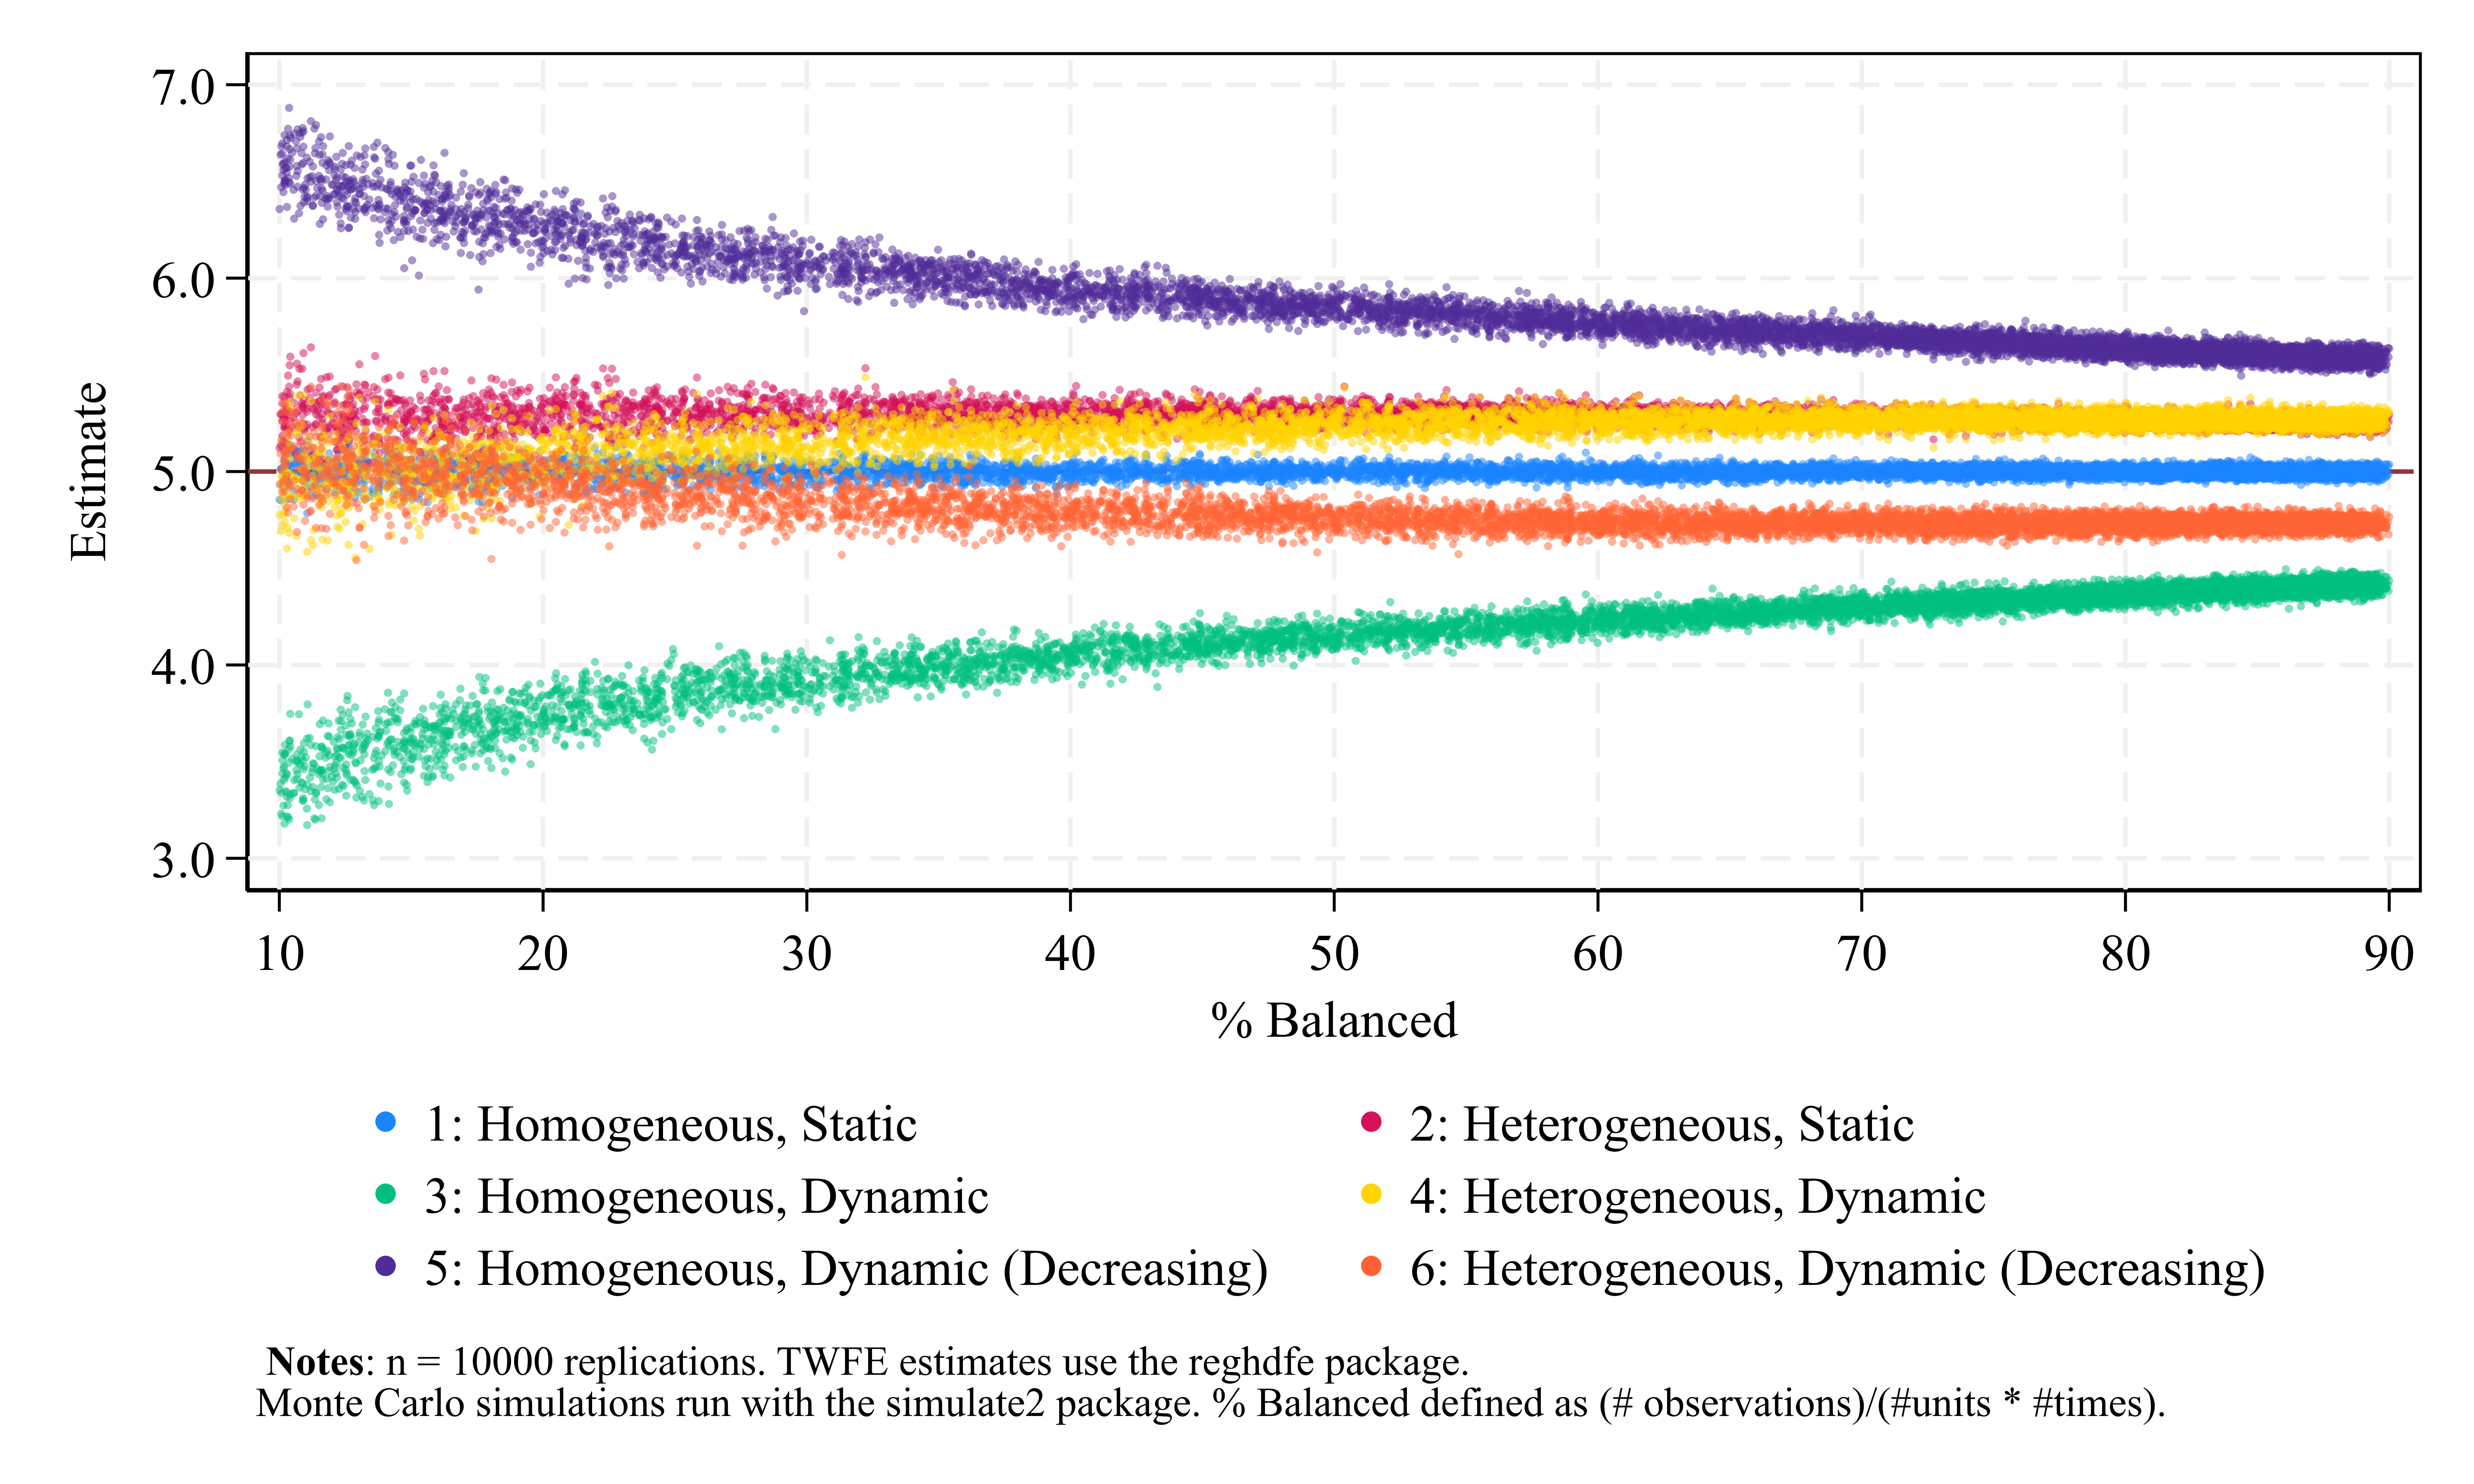
\includegraphics[width=5in]{Figures/TWFE Bias by Percent Balanced Scatter Crop.jpg}
    \label{fig:scatter-balance}
\end{figure}

\begin{figure}
    \centering
    \caption{Statistical Comparison of DiD Methods with True Average Effect by Percent Balanced (Relative Scale)}
    \includegraphics[width=6in]{Figures/Binscatters by Percent Balanced Common Scale.jpg}
    \label{fig:bins-balance-full}
\end{figure}

\begin{figure}
    \centering
    \caption{Statistical Comparison of DiD Methods with True Average Effect by Percent Balanced (Scatter Plot)}
    \includegraphics[width=6in]{Figures/Scatters by Percent Balanced Common Scale.jpg}
    \label{fig:scatters-common}
\end{figure}

\begin{figure}
    \centering
    \caption{Statistical Comparison of DiD Methods with True Average Effect by Percent Balanced (Scatter Plot) (Relative Scale)}
    \includegraphics[width=6in]{Figures/Scatters by Percent Balanced Relative Scale.jpg}
    \label{fig:scatters-relative}
\end{figure}

\begin{figure}[H]
    \centering
    \caption{Average Distribution of Data in Balanced and Unbalanced Simulations by Time Period and Treatment Status}
    \includegraphics[width=6.5in]{Figures/Average Distribution of Data in Simulations by Treated.jpg}
    \label{fig:dist-treat}
\end{figure}

To construct our sensitivity tables shown below, we randomly generate 50,000 regression datasets and run 6 TWFE models (for the 6 different treatment effects) on each one. The parameters we vary in the data are as follows:
\begin{center}
\begin{tabular}{r|l}
    Time periods ($T$) & $\{5, 10, \ldots, 50\}$ \\
    Units & $\{2500, 3000, \ldots, 5000\}$\\
    First cohort time ($T_{\text{start}}$) & $\{(T/5)+3, \ldots, T-1 \}$\\
    Last cohort time & $\{t_0+1, \ldots, T\}$\\
    \% Never Treated & \text{Uniform}(0, 1) \\
    \% Balanced & \hyperref[pcunbalancedfn]{\textbf{Described above}} \\
    True effect size & $\{-10, -9, \ldots, 10\}$\\
    Covariate size & \text{Uniform}(-5, 5) \\
\end{tabular}
\end{center}
There are two additional data modifiers. For 25\% of the datasets, we add an individual-specific treatment effect modifier.\footnote{The choice of 25\% is somewhat arbitrary, but allows for sufficient observations with the modifier turned on for inference, without introducing additional noise to most of our data.} This randomly adjusts the true treatment effect at the observation level by a mean-zero Normal distribution, where the standard deviation is randomly chosen as a function of the true effect size.\footnote{Specifically, the standard deviation $sd \sim |\text{Normal}(\text{True Effect}/10, |\text{True Effect}/2|)|$. We then draw from a Normal$(0, sd)$ distribution for each treated observation, and this draw is added to the \text{True Effect}.} Essentially, it adds noise to the true treatment effect at the observation level. Also, for 25\% of the datasets (independent of the individual-specific treatment effect modifier), we adjust our covariate by randomly picking a number from a standard Normal distribution, and adding that number to our covariate when $D_{it}=1$, inducing correlation between the covariate and treatment status. Summary statistics about the regression data are shown below.\footnote{39 out of 50,000 datasets are excluded from the regression. For these datasets, in the process of creating unbalanced data, all treated observations happen to be removed from the data. With no treated observations, the TWFE model is unidentified and so cannot be used in the regression. This does not appear to affect our results in any meaningful way.}

\begin{table}[htbp]\centering
\def\sym#1{\ifmmode^{#1}\else\(^{#1}\)\fi}
\caption{Summary Statistics of Sensitivity Regressions Data}
\label{tab:sensitivity-summary-stats}
\def\sym#1{\ifmmode^{#1}\else\(^{#1}\)\fi}
\begin{tabular}{l*{1}{cccccc}}
\hline\hline
                    &         $n$&        Mean&    Std.Dev.&      Median&         Min&         Max\\
\hline
Absolute Bias, Treatment Effect 1&      49,961&       0.242&       0.469&       0.040&       0.000&      13.054\\
Absolute Bias, Treatment Effect 2&      49,961&       0.450&       0.591&       0.208&       0.000&      13.054\\
Absolute Bias, Treatment Effect 3&      49,961&       1.114&       1.362&       0.637&       0.000&      17.037\\
Absolute Bias, Treatment Effect 4&      49,961&       1.771&       2.743&       0.818&       0.000&      33.894\\
Absolute Bias, Treatment Effect 5&      49,961&       1.114&       1.362&       0.637&       0.000&      16.995\\
Absolute Bias, Treatment Effect 6&      49,961&       1.771&       2.739&       0.822&       0.000&      33.834\\
Count of Units (1000s)&      49,961&       3.752&       0.853&       4.000&       2.500&       5.000\\
Count of Time Periods&      49,961&      27.471&      14.376&      30.000&       5.000&      50.000\\
\% Balanced         &      49,961&      64.541&      26.693&      73.158&       1.920&      96.128\\
\% Actively Treated &      49,961&      13.746&      12.413&      10.158&       0.001&      77.180\\
\% Never-Treated    &      49,961&      49.999&      28.697&      50.133&       0.000&      99.980\\
First Treatment Time&      49,961&      17.520&      10.757&      15.000&       4.000&      49.000\\
Last Treatment Time &      49,961&      22.989&      12.533&      22.000&       5.000&      50.000\\
Longest Treatment Exposure Time&      49,961&       9.951&       8.607&       7.000&       1.000&      37.000\\
True Effect Size    &      49,961&       0.003&       6.068&       0.000&     -10.000&      10.000\\
Individual-Specific Treatment Noise&      49,961&       0.344&       0.831&       0.000&       0.000&       4.995\\
Covariate Treatment Factor&      49,961&      -0.000&       0.503&       0.000&      -3.933&       3.679\\
Covariate Size      &      49,961&       0.005&       3.156&       0.000&      -5.000&       5.000\\
\hline\hline
\end{tabular}
\footnotesize  
\vspace{5mm}
    \footnotesize \begin{singlespace*}
        Each observation is the result of a TWFE model run on data which randomly changes the parameters shown here. `Absolute Bias' is the absolute difference between the TWFE model's estimated effect and the true average treatment effect on the treated (ATT) for a given dataset.
    \end{singlespace*}
\end{table}

\newgeometry{left=0.5in,bottom=0.5in,right=0.5in,top=0.5in,includefoot}

\begin{landscape}
\begin{table}[htbp]\centering
\def\sym#1{\ifmmode^{#1}\else\(^{#1}\)\fi}
\caption{Regressions of Absolute TWFE Bias}
\label{tab:sensitivity-table}
\scalebox{0.7}{
\begin{tabular}{l*{6}{c}}
\hline\hline
Dependent Variable: &\multicolumn{1}{c}{Data 1}&\multicolumn{1}{c}{Data 2}&\multicolumn{1}{c}{Data 3}&\multicolumn{1}{c}{Data 4}&\multicolumn{1}{c}{Data 5}&\multicolumn{1}{c}{Data 6}\\
 $|\text{Effect}_{TWFE} - \text{True Effect}|$ &Coefficient/SE         &Coefficient/SE         &Coefficient/SE         &Coefficient/SE         &Coefficient/SE         &Coefficient/SE         \\
\hline
\% Never-Treated    &      -0.001\sym{***}&      -0.002\sym{***}&      -0.050\sym{***}&      -0.112\sym{***}&      -0.050\sym{***}&      -0.112\sym{***}\\
                    &     (0.000)         &     (0.000)         &     (0.001)         &     (0.001)         &     (0.001)         &     (0.001)         \\
\% Never-Treated Squared&       0.000\sym{***}&       0.000\sym{***}&       0.000\sym{***}&       0.001\sym{***}&       0.000\sym{***}&       0.001\sym{***}\\
                    &     (0.000)         &     (0.000)         &     (0.000)         &     (0.000)         &     (0.000)         &     (0.000)         \\
Count of Units (1000s)&      -0.004         &       0.000         &      -0.008         &       0.001         &      -0.003         &      -0.003         \\
                    &     (0.002)         &     (0.003)         &     (0.006)         &     (0.011)         &     (0.006)         &     (0.011)         \\
Count of Time Periods&      -0.001\sym{***}&       0.007\sym{***}&       0.033\sym{***}&       0.099\sym{***}&       0.033\sym{***}&       0.099\sym{***}\\
                    &     (0.000)         &     (0.000)         &     (0.000)         &     (0.001)         &     (0.000)         &     (0.001)         \\
\% Balanced         &      -0.005\sym{***}&      -0.004\sym{***}&      -0.020\sym{***}&      -0.027\sym{***}&      -0.019\sym{***}&      -0.028\sym{***}\\
                    &     (0.000)         &     (0.000)         &     (0.001)         &     (0.002)         &     (0.001)         &     (0.002)         \\
\% Balanced Squared &       0.000\sym{***}&       0.000\sym{***}&       0.000\sym{***}&       0.000\sym{***}&       0.000\sym{***}&       0.000\sym{***}\\
                    &     (0.000)         &     (0.000)         &     (0.000)         &     (0.000)         &     (0.000)         &     (0.000)         \\
True Effect Size    &      -0.000         &      -0.000         &      -0.001         &       0.001         &      -0.001         &       0.000         \\
                    &     (0.000)         &     (0.000)         &     (0.001)         &     (0.002)         &     (0.001)         &     (0.002)         \\
Individual-Specific Treatment Noise&       0.007\sym{**} &      -0.001         &       0.001         &       0.004         &      -0.001         &       0.003         \\
                    &     (0.003)         &     (0.003)         &     (0.006)         &     (0.011)         &     (0.006)         &     (0.011)         \\
Covariate Treatment Factor&      -0.010\sym{*}  &       0.135\sym{***}&      -0.471\sym{***}&      -0.267\sym{***}&       0.453\sym{***}&       0.210\sym{***}\\
                    &     (0.004)         &     (0.005)         &     (0.010)         &     (0.018)         &     (0.010)         &     (0.018)         \\
Covariate Size      &      -0.000         &       0.000         &      -0.001         &      -0.003         &      -0.001         &      -0.003         \\
                    &     (0.001)         &     (0.001)         &     (0.002)         &     (0.003)         &     (0.002)         &     (0.003)         \\
Constant            &       0.430\sym{***}&       0.417\sym{***}&       2.453\sym{***}&       3.466\sym{***}&       2.424\sym{***}&       3.479\sym{***}\\
                    &     (0.015)         &     (0.018)         &     (0.035)         &     (0.065)         &     (0.035)         &     (0.065)         \\
\hline
Row Count           &   49961         &   49961         &   49961         &   49961         &   49961         &   49961         \\
Adjusted R Squared  &       0.011         &       0.045         &       0.337         &       0.444         &       0.334         &       0.445         \\
F Statistic         &      55.713         &     233.721         &    2535.005         &    3998.469         &    2501.697         &    4005.851         \\
Chi Squared p-value &       0.000         &       0.000         &       0.000         &       0.000         &       0.000         &       0.000         \\
\hline\hline
\multicolumn{7}{l}{\footnotesize \sym{*} \(p<0.05\), \sym{**} \(p<0.01\), \sym{***} \(p<0.001\)}\\
\end{tabular}
}
\footnotesize  
\vspace{5mm}
    \footnotesize \begin{singlespace*}
        Each observation in this regression is the result of a TWFE model run on data which randomly changes each of the parameters shown here. The dependent variable in this regression is the absolute difference between the TWFE model's estimated effect and the true average treatment effect on the treated (ATT).
    \end{singlespace*}
\end{table}
\end{landscape}
\begin{table}[htbp]\centering
\def\sym#1{\ifmmode^{#1}\else\(^{#1}\)\fi}
\caption{Regression Against Absolute Bias}
\begin{tabular}{l*{6}{c}}
\hline\hline
                    &\multicolumn{1}{c}{Data 1}&\multicolumn{1}{c}{Data 2}&\multicolumn{1}{c}{Data 3}&\multicolumn{1}{c}{Data 4}&\multicolumn{1}{c}{Data 5}&\multicolumn{1}{c}{Data 6}\\
                    &Coefficient/SE         &Coefficient/SE         &Coefficient/SE         &Coefficient/SE         &Coefficient/SE         &Coefficient/SE         \\
\hline
\% Never-Treated    &      -0.010\sym{***}&      -0.009\sym{***}&      -0.016\sym{***}&       0.046\sym{***}&      -0.015\sym{***}&       0.048\sym{***}\\
                    &     (0.002)         &     (0.002)         &     (0.004)         &     (0.007)         &     (0.004)         &     (0.007)         \\
\% Never-Treated Squared&       0.000\sym{***}&       0.000\sym{***}&       0.000\sym{***}&      -0.000\sym{**} &       0.000\sym{***}&      -0.000\sym{***}\\
                    &     (0.000)         &     (0.000)         &     (0.000)         &     (0.000)         &     (0.000)         &     (0.000)         \\
Count of Units (1000s)&       0.002         &       0.010         &      -0.022         &      -0.028         &      -0.013         &      -0.033         \\
                    &     (0.007)         &     (0.009)         &     (0.017)         &     (0.026)         &     (0.017)         &     (0.026)         \\
Count of Time Periods&      -0.002\sym{**} &       0.007\sym{***}&       0.084\sym{***}&       0.309\sym{***}&       0.084\sym{***}&       0.309\sym{***}\\
                    &     (0.001)         &     (0.001)         &     (0.001)         &     (0.002)         &     (0.001)         &     (0.002)         \\
\% Balanced         &      -0.006\sym{***}&      -0.007\sym{***}&      -0.036\sym{***}&      -0.067\sym{***}&      -0.036\sym{***}&      -0.065\sym{***}\\
                    &     (0.001)         &     (0.001)         &     (0.003)         &     (0.004)         &     (0.003)         &     (0.004)         \\
\% Balanced Squared &       0.000\sym{***}&       0.000\sym{***}&       0.000\sym{***}&       0.000\sym{***}&       0.000\sym{***}&       0.000\sym{***}\\
                    &     (0.000)         &     (0.000)         &     (0.000)         &     (0.000)         &     (0.000)         &     (0.000)         \\
True Effect Size    &      -0.001         &       0.000         &       0.000         &       0.008\sym{*}  &      -0.001         &       0.009\sym{*}  \\
                    &     (0.001)         &     (0.001)         &     (0.003)         &     (0.004)         &     (0.003)         &     (0.004)         \\
Individual-Specific Treatment Noise&       0.011         &       0.012         &       0.028         &       0.016         &       0.031         &       0.029         \\
                    &     (0.007)         &     (0.009)         &     (0.017)         &     (0.026)         &     (0.017)         &     (0.026)         \\
True Effect Size $\times$ Individual-Specific Treatment Noise&      -0.000         &      -0.001         &      -0.000         &      -0.000         &      -0.001         &       0.001         \\
                    &     (0.001)         &     (0.001)         &     (0.002)         &     (0.003)         &     (0.002)         &     (0.003)         \\
Covariate Treatment Factor&       0.010         &       0.044\sym{**} &      -0.737\sym{***}&      -0.498\sym{***}&       0.810\sym{***}&       0.401\sym{***}\\
                    &     (0.013)         &     (0.016)         &     (0.029)         &     (0.045)         &     (0.029)         &     (0.045)         \\
Covariate Size      &      -0.000         &       0.002         &      -0.003         &      -0.017\sym{*}  &      -0.004         &      -0.017\sym{*}  \\
                    &     (0.002)         &     (0.002)         &     (0.004)         &     (0.007)         &     (0.005)         &     (0.007)         \\
Covariate Treatment Factor $\times$ Covariate Size&       0.012\sym{**} &       0.013\sym{*}  &      -0.015         &      -0.047\sym{**} &      -0.014         &      -0.078\sym{***}\\
                    &     (0.004)         &     (0.005)         &     (0.009)         &     (0.015)         &     (0.009)         &     (0.015)         \\
\% Never-Treated $\times$ Count of Units (1000s)&      -0.000         &      -0.000         &       0.001         &       0.002         &       0.001         &       0.002         \\
                    &     (0.000)         &     (0.000)         &     (0.001)         &     (0.001)         &     (0.001)         &     (0.001)         \\
\% Never-Treated $\times$ Count of Time Periods&       0.000         &      -0.000         &      -0.002\sym{***}&      -0.007\sym{***}&      -0.002\sym{***}&      -0.007\sym{***}\\
                    &     (0.000)         &     (0.000)         &     (0.000)         &     (0.000)         &     (0.000)         &     (0.000)         \\
\% Never-Treated $\times$ \% Balanced&       0.000\sym{***}&       0.000\sym{***}&       0.001\sym{***}&       0.002\sym{***}&       0.001\sym{***}&       0.002\sym{***}\\
                    &     (0.000)         &     (0.000)         &     (0.000)         &     (0.000)         &     (0.000)         &     (0.000)         \\
\% Never-Treated $\times$ \% Balanced Squared&      -0.000\sym{***}&      -0.000\sym{***}&      -0.000\sym{***}&      -0.000\sym{***}&      -0.000\sym{***}&      -0.000\sym{***}\\
                    &     (0.000)         &     (0.000)         &     (0.000)         &     (0.000)         &     (0.000)         &     (0.000)         \\
\% Never-Treated $\times$ True Effect Size&      -0.000         &      -0.000         &      -0.000         &      -0.000\sym{*}  &      -0.000         &      -0.000\sym{*}  \\
                    &     (0.000)         &     (0.000)         &     (0.000)         &     (0.000)         &     (0.000)         &     (0.000)         \\
\% Never-Treated $\times$ Individual-Specific Treatment Noise&      -0.001\sym{*}  &      -0.001\sym{*}  &      -0.002\sym{*}  &      -0.001         &      -0.002\sym{*}  &      -0.002         \\
                    &     (0.000)         &     (0.000)         &     (0.001)         &     (0.001)         &     (0.001)         &     (0.001)         \\
\% Never-Treated $\times$ True Effect Size $\times$ Individual-Specific Treatment Noise&       0.000         &       0.000\sym{**} &       0.000         &       0.000         &       0.000         &       0.000         \\
                    &     (0.000)         &     (0.000)         &     (0.000)         &     (0.000)         &     (0.000)         &     (0.000)         \\
\% Never-Treated $\times$ Covariate Treatment Factor&      -0.002\sym{***}&       0.002\sym{*}  &       0.005\sym{***}&       0.003         &      -0.010\sym{***}&      -0.002         \\
                    &     (0.001)         &     (0.001)         &     (0.001)         &     (0.002)         &     (0.001)         &     (0.002)         \\
\% Never-Treated $\times$ Covariate Size&       0.000         &      -0.000         &       0.000         &       0.001\sym{*}  &       0.000         &       0.001\sym{*}  \\
                    &     (0.000)         &     (0.000)         &     (0.000)         &     (0.000)         &     (0.000)         &     (0.000)         \\
\% Never-Treated $\times$ Covariate Treatment Factor $\times$ Covariate Size&      -0.001\sym{***}&      -0.001\sym{**} &       0.000         &       0.002\sym{*}  &       0.000         &       0.002\sym{***}\\
                    &     (0.000)         &     (0.000)         &     (0.000)         &     (0.001)         &     (0.000)         &     (0.001)         \\
\% Never-Treated Squared $\times$ Count of Units (1000s)&      -0.000         &       0.000         &      -0.000         &      -0.000         &      -0.000         &      -0.000         \\
                    &     (0.000)         &     (0.000)         &     (0.000)         &     (0.000)         &     (0.000)         &     (0.000)         \\
\% Never-Treated Squared $\times$ Count of Time Periods&      -0.000         &       0.000         &       0.000\sym{***}&       0.000\sym{***}&       0.000\sym{***}&       0.000\sym{***}\\
                    &     (0.000)         &     (0.000)         &     (0.000)         &     (0.000)         &     (0.000)         &     (0.000)         \\
\% Never-Treated Squared $\times$ \% Balanced&      -0.000\sym{***}&      -0.000\sym{***}&      -0.000\sym{***}&      -0.000\sym{***}&      -0.000\sym{***}&      -0.000\sym{***}\\
                    &     (0.000)         &     (0.000)         &     (0.000)         &     (0.000)         &     (0.000)         &     (0.000)         \\
\% Never-Treated Squared $\times$ \% Balanced Squared&       0.000\sym{***}&       0.000\sym{***}&       0.000\sym{***}&       0.000\sym{***}&       0.000\sym{***}&       0.000\sym{***}\\
                    &     (0.000)         &     (0.000)         &     (0.000)         &     (0.000)         &     (0.000)         &     (0.000)         \\
\% Never-Treated Squared $\times$ True Effect Size&       0.000         &       0.000         &       0.000         &       0.000\sym{*}  &       0.000         &       0.000\sym{*}  \\
                    &     (0.000)         &     (0.000)         &     (0.000)         &     (0.000)         &     (0.000)         &     (0.000)         \\
\% Never-Treated Squared $\times$ Individual-Specific Treatment Noise&       0.000\sym{**} &       0.000\sym{**} &       0.000\sym{**} &       0.000         &       0.000\sym{*}  &       0.000\sym{*}  \\
                    &     (0.000)         &     (0.000)         &     (0.000)         &     (0.000)         &     (0.000)         &     (0.000)         \\
\% Never-Treated Squared $\times$ True Effect Size $\times$ Individual-Specific Treatment Noise&      -0.000\sym{*}  &      -0.000\sym{**} &      -0.000         &      -0.000         &      -0.000         &      -0.000         \\
                    &     (0.000)         &     (0.000)         &     (0.000)         &     (0.000)         &     (0.000)         &     (0.000)         \\
\% Never-Treated Squared $\times$ Covariate Treatment Factor&       0.000\sym{***}&       0.000         &       0.000         &       0.000         &       0.000\sym{***}&      -0.000         \\
                    &     (0.000)         &     (0.000)         &     (0.000)         &     (0.000)         &     (0.000)         &     (0.000)         \\
\% Never-Treated Squared $\times$ Covariate Size&      -0.000         &       0.000         &      -0.000         &      -0.000\sym{*}  &      -0.000         &      -0.000\sym{*}  \\
                    &     (0.000)         &     (0.000)         &     (0.000)         &     (0.000)         &     (0.000)         &     (0.000)         \\
\% Never-Treated Squared $\times$ Covariate Treatment Factor $\times$ Covariate Size&       0.000\sym{***}&       0.000\sym{**} &      -0.000         &      -0.000\sym{*}  &      -0.000         &      -0.000\sym{**} \\
                    &     (0.000)         &     (0.000)         &     (0.000)         &     (0.000)         &     (0.000)         &     (0.000)         \\
Constant            &       0.456\sym{***}&       0.425\sym{***}&       1.232\sym{***}&      -1.380\sym{***}&       1.184\sym{***}&      -1.411\sym{***}\\
                    &     (0.041)         &     (0.051)         &     (0.092)         &     (0.143)         &     (0.093)         &     (0.143)         \\
\hline
Row Count           &   49961.000         &   49961.000         &   49961.000         &   49961.000         &   49961.000         &   49961.000         \\
Adjusted R Squared  &       0.016         &       0.050         &       0.403         &       0.647         &       0.399         &       0.647         \\
F Statistic         &      26.817         &      83.462         &    1054.185         &    2856.657         &    1037.056         &    2857.664         \\
Chi Squared p-value &       0.000         &       0.000         &       0.000         &       0.000         &       0.000         &       0.000         \\
\hline\hline
\multicolumn{7}{l}{\footnotesize \sym{*} \(p<0.05\), \sym{**} \(p<0.01\), \sym{***} \(p<0.001\)}\\
\end{tabular}
\end{table}

\end{document}